%% ============================================================
%% EvoRiri - COMPLETE CORRECTED main.tex
%%   1. Journal name: mathematics
%%   2. PNG logo (XeTeX-compatible)
%%   3. COI disclosure updated
%%   4. Conclusions sentence completed
%%   5. \DeclareGraphicsExtensions added
%%   6. \externaleditor cleared (COI)
%% ============================================================

\documentclass[mathematics,article,xetex,moreauthors]{Definitions/mdpi}
%% NOTE: 'submit' option temporarily removed to isolate a lineno/cleveref
%% "Runaway definition of \@LN@column" compile error. 'submit' is what
%% triggers MDPI's line-numbering via the lineno package. If this version
%% compiles cleanly, the error is confirmed to originate in lineno's
%% interaction with this TeX Live install, not in the paper content.
%% Re-add 'submit' only once that's resolved (e.g. via MDPI support or a
%% lineno/cleveref package update), since MDPI requires line numbers for
%% actual submission.
\usepackage{fontspec}
\setlength{\headheight}{20pt}
\addtolength{\topmargin}{-8pt}
\usepackage{tikz}
\usetikzlibrary{arrows.meta, positioning, fit}
\emergencystretch=2em
\newfontfamily\bengalifont[Script=Bengali]{Noto Serif Bengali}
\pubvolume{1}
\issuenum{1}
\articlenumber{0}
\pubyear{2026}
\copyrightyear{2026}
%% Supervisor is Guest Editor of this Special Issue; COI disclosed to MDPI prior to submission
%% \externaleditor left blank; disclose COI to editorial office before submission
\datereceived{}
\daterevised{}
\dateaccepted{}
\datepublished{}
\hreflink{https://doi.org/}

\Title{EvoRiri: Risk-Aware Genetic Optimization of a Safety-First,
Empathetic Bangla Mental-Health Assistant}

\TitleCitation{Risk-Aware Genetic Optimization of Mental-Health Responses}

%% ORCID: only M.M.J. Kabir's is currently on file; add Rahman's here
%% (\newcommand{\orcidauthorA}{...}) once available.
\newcommand{\orcidauthorB}{0000-0003-4963-8905}

\Author{Jahnnobi Rahman $^{1}$ and Mir Md.\ Jahangir Kabir $^{2,}$*\orcidB{}}
\AuthorNames{Jahnnobi Rahman and Mir Md. Jahangir Kabir}
\AuthorCitation{Author, F.; Author, S.; Author, T.}

\address[1]{Relaxy PTE. LTD., Singapore , Bangladesh; jahnnobirahman230@gmail.com}
\address[2]{University of Technology Sydney, 15 Broadway, Ultimo NSW 2007, Australia; mirmdjahangir.kabir@uts.edu.au}

\corres{Correspondence: jahnnobirahman230@gmail.com}

\abstract{Large language models are increasingly deployed in emotionally sensitive applications
such as mental-health support, where optimization must jointly consider empathy, safety, and
conversational structure. We present a genetic-algorithm (GA) framework for optimizing the
response-generation policy of \textit{Riri}, a Bangla/Banglish/English mental-health assistant. Instead of
updating model weights, the GA searches over an interpretable genome that parametrizes response
structure and style within a risk-aware, template-based generator that requires no LLM calls at
deployment. A non-differentiable fitness function combines
automatic scores for empathy, safety, and structure, subject to hard safety constraints and smooth
penalty terms. Experiments on a corpus of 2872 de-identified prompts with suicide-risk labels
show that the GA converges rapidly to high-fitness policies, improving structural completeness
by more than a factor of forty in our setting relative to an unoptimized baseline, substantially improving safety,
and slightly increasing empathy. Performance appears effectively stable beyond approximately 300--600
training prompts under our experimental configuration, indicating that moderate datasets may suffice to provide a stable optimization signal.
Trace analysis reveals typical evolutionary failure modes including question-only structural collapse
and empathy marker stuffing and demonstrates how revised scoring and progressive structure
enforcement steer search toward behaviorally meaningful responses. The results highlight both the
promise and the pitfalls of evolutionary optimization for value-laden conversational AI.}

\keyword{evolutionary algorithms; genetic algorithms; mental-health chatbots;
large language models; empathy; safety; multi-objective optimization;
conversational agents; Bangla; risk-aware AI}


%%%%%%%%%%%%%%%%%%%%%%%%%%%%%%%%%%%%%%%%%%%%%%%%%%%%%%%%%%%%
\begin{document}
%%%%%%%%%%%%%%%%%%%%%%%%%%%%%%%%%%%%%%%%%%%%%%%%%%%%%%%%%%%%

\section{Introduction}

Large language models (LLMs) are increasingly used as conversational agents in
domains such as mental-health support, coaching, and
counseling~\cite{jmir2025_chatbots,pmc2026_chatbots}. Deploying these systems
safely requires more than grammatical correctness or task accuracy; responses
must be empathetic, structurally helpful, and aligned with risk-aware safety
principles~\cite{jmir2024_empathic,apa2024_advisory,harvard2024_safety}.

Conventional fine-tuning and reinforcement learning from human feedback (RLHF)
are powerful but expensive and tightly coupled to model weights. In contrast,
evolutionary algorithms (EAs) can optimize high-level, interpretable policies
using arbitrary non-differentiable
objectives~\cite{llm_ea_survey2025,when_llms_meet_ea2025}. In the context of
conversational agents, this makes them attractive for optimizing template-based
generators or routing strategies while keeping the underlying LLM
fixed~\cite{mles2026,gendl2025}.

Unlike prior evolutionary prompt optimization approaches that focus primarily on
reasoning accuracy, feature activation, or prompt engineering, the proposed
framework focuses on optimizing emotionally sensitive conversational behavior
under explicit safety constraints. The system introduces risk-aware escalation,
progressive structure enforcement, and trace-level behavioral analysis for a
multilingual mental-health assistant. To the best of our knowledge, this is
among the first studies applying interpretable genetic optimization to
empathy--safety--structure balancing in Bangla mental-health conversational
systems.

In this article we introduce an evolutionary optimization framework for
\emph{Riri}, a mental-health-oriented assistant designed for Bangla-speaking
users. The system wraps the LLM in a structured generator that controls when to
include empathy, grounding, action suggestions, and reflective questions. A
genetic algorithm (GA) evolves a genome of continuous and discrete parameters
that govern this generator. The optimization objective aggregates scores for
empathy, safety, and structure under explicit constraints for suicide and
self-harm risk.

The main contributions of this work are:
\begin{itemize}
  \item A risk-aware GA formulation for mental-health response generation,
        including an interpretable genome, progressively structured generator,
        and constrained fitness.
  \item An empirical study of GA convergence, data efficiency, and
        population-size sensitivity on a corpus of 2872 de-identified
        mental-health prompts with risk labels.
  \item A trace-based analysis of evolutionary failure modes (structural
        collapse, empathy overfitting) and demonstration of how revised scoring
        and hard constraints yield behaviorally meaningful responses.
\end{itemize}

The novelty of this work lies not only in applying a GA to response generation,
but in using evolutionary search to optimize safety-critical conversational
behavior under interpretable constraints. The framework combines risk-aware
escalation, progressive structure enforcement, and trace-based failure analysis.
This enables the study to examine how evolutionary systems behave when
optimizing value-laden objectives such as empathy, safety, and structured
support.

The rest of the paper is organized as follows.
Section~\ref{sec:related} reviews related work.
Section~\ref{sec:methods} describes the dataset, genome, generator, and fitness
function.
Section~\ref{sec:results} presents experimental results.
Section~\ref{sec:discussion} discusses implications and limitations, and
Section~\ref{sec:conclusion} concludes.

\subsection{Research Hypotheses}

This study evaluates the following hypotheses:

\textbf{H1:} Genetic Algorithm optimization improves overall response quality
compared with the baseline response generator.

\textbf{H2:} Progressive structure enforcement improves structural completeness
without substantially reducing safety.

\textbf{H3:} Moderate dataset sizes provide a sufficiently stable fitness
signal for GA-based response optimization.

\textbf{H4:} Larger GA populations improve optimization stability up to an
intermediate range, after which performance gains diminish.

\textbf{H5:} Hard safety constraints reduce unsafe or inappropriate
optimization shortcuts in high-risk mental-health contexts.

%%%%%%%%%%%%%%%%%%%%%%%%%%%%%%%%%%%%%%%%%%%%%%%%%%%%%%%%%%%%
\section{Related Work}
\label{sec:related}

\subsection{Evolutionary Algorithms for LLM and Prompt Optimization}

Recent research has increasingly explored the integration of Evolutionary
Algorithms (EAs) with Large Language Models (LLMs) for optimization, reasoning,
and controllable generation tasks. A growing body of work suggests that
evolutionary search provides a promising alternative to gradient-based alignment
methods, particularly in black-box API settings where direct model fine-tuning
is impractical.

The survey ``When Large Language Models Meet Evolutionary
Algorithms''~\cite{when_llms_meet_ea2025} establishes a conceptual bridge
between token-sequence generation in LLMs and population-based search in
evolutionary systems. The authors argue that prompts, policies, and language
structures can be treated as evolvable individuals within an optimization
landscape. Their framework motivates the use of mutation, crossover, and fitness
shaping in language-space optimization. The present work follows this paradigm
by treating conversational behavior policies as evolvable genomes composed of
interpretable parameters such as empathy weight, safety weight, structure
weight, escalation thresholds, and template configurations.

Similarly, Promptbreeder~\cite{epo2025} proposes a self-referential
prompt evolution framework in which mutation operators are themselves
evolved alongside the prompts. Promptbreeder demonstrates that genetic
search can discover diverse, high-performing prompts across reasoning
tasks without manual engineering. While Promptbreeder targets task
accuracy, the proposed framework extends the evolutionary optimization
paradigm toward safety-critical conversational behavior.

GAAPO~\cite{gaapo2025} further demonstrates the effectiveness of Genetic
Algorithms for automatic prompt optimization in LLM systems. Their work explores
mutation, crossover, selection strategies, and population hyperparameter
trade-offs across benchmark reasoning tasks such as ETHOS, MMLU-Pro, and GPQA.
Similar to GAAPO, the present study investigates population-size and
dataset-size sensitivity in evolutionary optimization. However, unlike GAAPO,
the proposed framework focuses on multi-objective optimization for mental-health
dialogue systems, balancing empathy, safety, structural completeness, and
conversational naturalness.

GenDLN~\cite{gendl2025} applies evolutionary optimization to stacked LLM
reasoning pipelines using non-differentiable objectives. The work demonstrates
that GA-based optimization can effectively operate over black-box API systems
without gradient access. However, GenDLN primarily targets logical reasoning and
classification performance, whereas the present work investigates emotionally
sensitive conversational optimization under safety constraints.

Another closely related direction is Multimodal LLM-assisted Evolutionary
Search (MLES)~\cite{mles2026}, which combines LLM reasoning with evolutionary
optimization to generate interpretable programmatic control policies. MLES
emphasizes behavioral evidence and transparent policy evolution rather than
relying solely on scalar reward signals.

A recent systematic survey on LLMs for Evolutionary
Optimization~\cite{llm_ea_survey2025} categorizes hybrid EA-LLM systems into
low-level and high-level optimization frameworks. The proposed framework belongs
primarily to the low-level LLM-assisted optimization category, where
evolutionary search operates directly over interpretable conversational policies.

Overall, existing EA+LLM research primarily focuses on reasoning accuracy,
feature activation, program synthesis, or prompt engineering. The proposed work
contributes to this emerging direction by introducing a risk-aware,
multi-objective GA framework for mental-health conversational optimization.

\subsection{Mental-Health Conversational Agents}

Mental-health chatbots and conversational agents have received significant
attention in recent years due to their potential to provide scalable
psychological support. Systematic
reviews~\cite{jmir2025_chatbots,pmc2026_chatbots} suggest that generative
conversational agents can improve emotional accessibility and user engagement,
particularly among populations with limited access to professional mental-health
care.

Recent work on empathic conversational agent design~\cite{jmir2024_empathic}
highlights the importance of empathy, conversational structure, and safety
mechanisms in determining user trust and therapeutic effectiveness. These
findings directly motivate the three-dimensional optimization objective used in
the proposed framework: empathy, safety, and structural support.

Emotionally intelligent chatbot systems have also raised important ethical and
safety concerns~\cite{ijca2025emotion}. Prior studies emphasize that emotionally
persuasive conversational systems can unintentionally produce unsafe or
misleading outputs if optimization objectives are poorly specified.

Other mental-health chatbot systems have relied primarily on sentiment analysis
and rule-based support generation~\cite{scitepress2025chatbot}. In contrast, the
proposed framework employs evolutionary optimization to dynamically shape
conversational behavior based on fitness feedback.

The American Psychological Association (APA) advisory on generative AI for
mental health~\cite{apa2024_advisory} further stresses the necessity of explicit
safety constraints and escalation policies in AI mental-health systems.

Empirical studies on the safety of generative AI chatbots in mental-health
contexts~\cite{harvard2024_safety} also demonstrate that conversational agents
may exhibit inconsistent crisis behavior when not explicitly constrained.

Human-AI collaborative mental-health systems~\cite{humanai2024} have
additionally shown that empathy and conversational structure significantly
influence perceived support quality.

\subsection{Empathy Modeling and Conversational Behavior Optimization}

Empathy modeling has become an increasingly important area within conversational
AI research. Surveys on artificial empathy
classification~\cite{empathysurvey2025} discuss various methods for evaluating
empathetic language using linguistic markers, neural scoring systems, and
psychological frameworks. The present work adopts a lightweight rubric-based
evaluation approach due to its interpretability and compatibility with black-box
optimization settings.

Neural empathetic conversational systems~\cite{empatheticagents2025} have
demonstrated strong performance in emotionally aware dialogue generation, but
these methods often require large-scale supervised training and expensive
fine-tuning pipelines. In contrast, the proposed framework explores whether
evolutionary search over interpretable conversational policies can improve
empathetic behavior without retraining the underlying LLM.

Research on conversational trust and chatbot
evolution~\cite{chatbotevolution2024} further suggests that users respond more
positively to systems exhibiting balanced empathy, clear structure, and
contextual appropriateness.

\subsection{Research Gap and Positioning}

Existing studies on evolutionary prompt optimization primarily focus on
improving reasoning performance, feature activation, or general task accuracy.
Similarly, prior mental-health conversational systems often emphasize either
empathy or safety independently, with limited attention to structural balance
and risk-aware escalation. There remains a gap in developing interpretable
optimization frameworks that jointly balance empathy, safety, structure, and
adaptive risk-sensitive behavior in multilingual mental-health support systems.

\begin{table}[H]
\centering
\caption{Comparison of the proposed framework with related approaches.}
\label{tab:related-comparison}
\renewcommand{\arraystretch}{1.2}
\begin{tabularx}{\textwidth}{
  >{\raggedright\arraybackslash}p{3.8cm}
  >{\centering\arraybackslash}p{1.3cm}
  >{\centering\arraybackslash}p{1.5cm}
  >{\centering\arraybackslash}p{1.5cm}
  >{\centering\arraybackslash}p{1.7cm}
  >{\centering\arraybackslash}p{1.8cm}
}
\toprule
\textbf{Approach} & \textbf{GA/EA} & \textbf{Empathy} &
\textbf{Safety} & \textbf{Structure} & \textbf{Risk-aware} \\
\midrule
Rule-based mental-health chatbots
  & No & Partial & Partial & Partial & Partial \\
LLM-based mental-health assistants
  & No & Yes & Partial & Partial & Partial \\
RLHF-based alignment methods
  & No & Yes & Yes & Limited & Partial \\
GA-based prompt optimization (e.g., Promptbreeder, GAAPO)
  & Yes & Limited & Limited & Limited & No \\
\rowcolor{gray!10}\textbf{Proposed framework}
  & \textbf{Yes} & \textbf{Yes} & \textbf{Yes} & \textbf{Yes} & \textbf{Yes} \\
\bottomrule
\end{tabularx}
\end{table}

As shown in Table~\ref{tab:related-comparison}, existing approaches typically
optimize either conversational quality or alignment objectives independently. In
contrast, the proposed framework jointly optimizes empathy, safety, structural
coherence, and risk-aware escalation within a unified evolutionary optimization
framework.

%%%%%%%%%%%%%%%%%%%%%%%%%%%%%%%%%%%%%%%%%%%%%%%%%%%%%%%%%%%%
\section{Methodology}
\label{sec:methods}

\subsection{Problem Formulation}

Let \(X\) denote the space of user prompts and
\(R = \{\mathrm{low}, \mathrm{mid}, \mathrm{high}\}\) the set of
suicide/self-harm risk labels. A response-generation policy is a function
\begin{equation}
  \pi_{\theta} : X \times R \rightarrow Y,
\end{equation}
mapping a prompt \(x \in X\) with risk \(r \in R\) to a textual response
\(y \in Y\). Instead of optimizing LLM parameters directly, we parameterize
\(\pi_{\theta}\) via a higher-level generator \(G\) controlled by a genome
\(g \in \mathcal{G}\):
\begin{equation}
\label{eq:generator}
  y = G(x, r; g).
\end{equation}
The design goal is to find a genome \(g^{\star}\) that maximizes a scalar
fitness function \(F(g)\) combining empathy, safety, and structure:
\begin{equation}
\label{eq:objective}
  g^{\star} = \arg\max_{g \in \mathcal{G}} F(g)
  \quad \text{subject to safety constraints}.
\end{equation}
We approximate~\eqref{eq:objective} using a GA operating on a finite set of
prompts.


\begin{figure}[H]
  \centering
  \begin{tikzpicture}[
      node distance=10mm,
      box/.style={rectangle, rounded corners, draw, minimum width=4.8cm,
                  minimum height=1.3cm, align=center, font=\small},
      arr/.style={-{Latex[length=2mm]}, thick}
  ]
  
  \node[box] (prompt) {User prompt + risk label\\[1pt] \footnotesize $(x_i, r_i)$};
  \node[box, below=of prompt] (genome) {Genome $g$\\[1pt] \footnotesize Weights \& thresholds, Eq.~\eqref{eq:genome}};
  \node[box, below=of genome] (generator) {Generator $G$\\[1pt] \footnotesize Template composer, Eq.~\eqref{eq:generator}};
  \node[box, below=of generator] (response) {Response $y_i$\\[1pt] \footnotesize $y_i = G(x_i,r_i;g)$};
  \node[box, below=of response] (scoring) {Automatic scoring\\[1pt] \footnotesize $E_i,S_i,C_i$, Eqs.~\eqref{eq:empathy}--\eqref{eq:structure}};
  \node[box, below=of scoring] (fitness) {Fitness $F(g)$\\[1pt] \footnotesize Eqs.~\eqref{eq:per-example}--\eqref{eq:global}};
  
  \draw[arr] (prompt) -- (genome);
  \draw[arr] (genome) -- (generator);
  \draw[arr] (generator) -- (response);
  \draw[arr] (response) -- (scoring);
  \draw[arr] (scoring) -- (fitness);
  
  % Feedback loop: GA evolves the genome based on fitness
  \draw[arr, dashed] (fitness.east) -- ++(1.7cm,0) |- (genome.east)
      node[midway, right, font=\footnotesize, align=left, xshift=1mm]
      {GA evolves $g$\\via Eq.~\eqref{eq:objective}};
  
  \end{tikzpicture}
  \caption{Overview of the EvoRiri response-generation and optimization pipeline,
  with the governing equation shown for each stage. A genome $g$
  (Eq.~\eqref{eq:genome}) parametrizes the template-based generator $G$
  (Eq.~\eqref{eq:generator}), which produces a response $y_i$ for each
  prompt-risk pair $(x_i, r_i)$. Automatic scoring
  (Eqs.~\eqref{eq:empathy}--\eqref{eq:structure}) yields the per-example and
  global fitness (Eqs.~\eqref{eq:per-example}--\eqref{eq:global}), which the
  genetic algorithm uses to evolve the genome via the objective in
  Eq.~\eqref{eq:objective}.}
  \label{fig:pipeline}
  \end{figure}

\paragraph{Worked example.} To make the abstract pipeline in
Figure~\ref{fig:pipeline} concrete, we walk a single prompt through every
stage using the converged genome $g^{\star}$ from Table~\ref{tab:hyperparams-ga}
($w_e^{\star}=0.137$, $w_s^{\star}=0.086$, $w_c^{\star}=0.778$,
$\theta_{\mathrm{mid}}^{\star}=0.700$, $\theta_{\mathrm{high}}^{\star}=0.731$).

\begin{enumerate}
  \item \textbf{Prompt + risk label.} $x_i = $ ``Ami onek lonely feel kortesi
        lately. I feel really anxious and overwhelmed.'' For illustration we
        take $r_i = \mathrm{mid}$.
  \item \textbf{Genome.} The generator is configured with $g^{\star}$ as
        above (Eq.~\eqref{eq:genome}).
  \item \textbf{Generator.} Because $w_c^{\star}=0.778$ falls in the top
        structure regime ($w_c \ge 0.55$; Section~\ref{sec:progressive-structure}),
        the generator deterministically includes grounding, action, and
        question components ($c_g=c_a=c_q=1$); $w_e^{\star}$ and
        $w_s^{\star}$ govern how many empathy lines and how conservative the
        phrasing is.
  \item \textbf{Response.} $y_i = G(x_i,r_i;g^{\star}) = $ ``Feeling this
        alone can be really painful. {\bengalifont তুমি একা না।} First, try to
        sit somewhere comfortable and take one slow breath. Try not to stay
        completely isolated with these thoughts. Is there someone nearby you
        feel comfortable talking to?'' (the same post-fix response reported
        in Appendix~A.3 for this prompt).
  \item \textbf{Automatic scoring.} This response receives
        $E_i = 0.45$, $S_i = 1.00$, $C_i = 1.00$
        (Eqs.~\eqref{eq:empathy}--\eqref{eq:structure}), reflecting one
        focused reflective question alongside the grounding and action
        content rather than the question-only collapse described in
        Appendix~A.1.
  \item \textbf{Fitness.} The response is below the 140-word penalty
        threshold, so $L_i=0$; the risk label is mid and $S_i=1.00 \ge 0.94$,
        so neither flat penalty applies; $C_i=1.00 \ge 0.70$, so the
        structure soft penalty does not apply; $E_i=0.45 < 0.62$, so the
        empathy soft penalty does apply. The per-example fitness
        (Eq.~\eqref{eq:per-example-fitness}) is
        \begin{align*}
          f_i(g^{\star}) &= \underbrace{0.40(0.45) + 0.40(1.00) + 0.15(1.00)}_{\text{base } A E_i+B S_i+C C_i}
            \;-\; \underbrace{0.18\,\tfrac{0.62-0.45}{0.62}}_{\text{empathy soft penalty}} \\
            &\quad + \underbrace{0.05(0.45) + 0.05(1.00) + 0.05\min(1.00,0.8)}_{\text{reinforcement terms}} \\
            &\approx 0.730 - 0.049 + 0.023 + 0.05 + 0.04 = 0.793.
        \end{align*}
        Averaging $f_i(g^{\star})$ over the $|\mathcal{I}|=600$ sampled
        prompts in a generation (Eq.~\eqref{eq:global}) gives the reported
        validation fitness $F(g^{\star}) \approx 0.678$
        (Table~\ref{tab:baseline-optimized}); the single-example value above
        is higher than this average, as expected for one example already
        matching the converged genome's dominant behaviour (full structure)
        while other sampled prompts and risk levels contribute lower
        per-example scores to the mean.
  \item \textbf{GA feedback.} Across generations, genomes whose responses
        score well on this fitness are more likely to be selected, crossed
        over, and mutated into the next population
        (Section~\ref{sec:ga-config}), which is how the search arrived at
        $g^{\star}$ from the seeded initial population (Appendix~B).
\end{enumerate}

\subsection{Dataset}

We use a dataset of \(N = 2872\) de-identified prompts collected from a
mental-health screening and support application in Bangladesh. Each example
\(i \in \{1,\dots,N\}\) consists of:
\begin{equation}
  (x_i, r_i, t_i),
\end{equation}
where \(x_i\) is the user message in Bangla, Banglish, or English;
\(r_i \in R\) is the risk label (low, mid, high); and \(t_i\) is a high-level
theme description (e.g., economic stress, relationship issues, suicidal
ideation) used only for analysis~\cite{jmir2025_chatbots}.

For some experiments we consider subsets of size
\(N_s \in \{100, 300, 600, 1200, 2872\}\) to study data efficiency. Each subset
is split into an optimization set and a held-out validation set using an
80/20 split, stratified by risk label so that the proportion of low-, mid-,
and high-risk prompts in the validation set matches the proportion in the
full subset. For the main experiment ($N_s = 2872$), this yields
approximately 2,297 optimization prompts and 575 validation prompts, with
fitness evaluation during GA optimisation performed on a random sample of
$|\mathcal{I}| = 600$ prompts drawn from the optimization set per generation
(Table~\ref{tab:hyperparams-ga}).

\subsection{Genome Representation}

An individual genome \(g\) is a vector of continuous and discrete genes:
\begin{equation}
\label{eq:genome}
  g = \bigl( w_e,\, w_s,\, w_c,\, \theta_{\mathrm{mid}},\,
             \theta_{\mathrm{high}},\, \lambda,\, d \bigr),
\end{equation}
where:
\begin{itemize}
  \item \(w_e \in [0,1]\): empathy weight controlling the number and intensity
        of empathy lines.
  \item \(w_s \in [0,1]\): safety weight. In the present implementation it
        selects one of several internal safety-instruction annotations that
        are stripped before the response is finalised, so it does not
        currently influence the visible response text or any automatic score;
        crisis-language inclusion is instead governed directly by the risk
        label (Section~\ref{sec:risk-escalation}).
  \item \(w_c \in [0,1]\): structure weight controlling inclusion of grounding,
        action, and questions.
  \item \(\theta_{\mathrm{mid}}, \theta_{\mathrm{high}} \in [0,1]\): reserved
        risk-escalation thresholds. They are part of the genome and are
        subject to crossover and mutation like every other gene, but in the
        present implementation they are not read by the generator or the
        fitness function, and therefore have no effect on any reported result.
        We retain them in the genome because they are the intended interface
        for the graded, distress-score-driven escalation described as future
        work in Section~\ref{sec:limitations}.
  \item \(\lambda \in [0,1]\): length penalty coefficient.
  \item \(d\): discrete template selector, indexing a small set of response
        templates.
\end{itemize}

To establish a meaningful performance reference, we define three baseline
conditions. The zero-shot baseline (B1) instantiates the generator with
minimum genome weights ($w_e = w_s = w_c = 0.10$, $\lambda = 0$), a short
memory window of 256 tokens, and maximally conservative escalation thresholds
($\theta_\mathrm{mid} = 0.70$, $\theta_\mathrm{high} = 0.95$), representing
response generation with no parameter optimisation. The fixed seed baseline
(B2) uses the balanced initialisation genome $g_\mathrm{bal}$ without
evolutionary search, isolating the contribution of the search process itself.
The random baseline (B3) averages five genomes sampled uniformly from the
genome space, establishing a chance-level reference.

\subsection{Risk-Aware Generator}
\label{sec:generator}

The generator \(G\) composes responses from several component banks:
\begin{itemize}
  \item Empathy lines (Bangla/Banglish/English) expressing emotional validation.
  \item Grounding instructions (e.g., breathing, 5-4-3-2-1 sensory exercise).
  \item Action suggestions (e.g., contact trusted friend, seek professional
        help).
  \item Reflective questions encouraging further disclosure.
\end{itemize}

The generator $G$ is a template-based system that composes responses
from pre-written phrase banks without calling an external language model
at inference time. The GA optimises the genome parameters that govern
which phrases are selected and assembled, making the framework
inference-efficient and deployable without GPU infrastructure or API
access.

\subsubsection{Progressive Structure Enforcement}
\label{sec:progressive-structure}

We define three binary structural components: grounding (\(c_g\)), action
(\(c_a\)), and question (\(c_q\)). Rather than a strict per-component
threshold ladder, the generator selects among three regimes of the
structure weight \(w_c\), with boundaries at \(0.25\) and \(0.55\):
\begin{itemize}
  \item \(w_c < 0.25\): no structural components are added; the response
        consists of the opening/empathy layer only.
  \item \(0.25 \le w_c < 0.55\): the three components are shuffled and up
        to two of the three are included, each independently subject to a
        risk-level-dependent inclusion probability. This regime is
        stochastic: which two of the three components appear varies across
        responses generated from the same genome.
  \item \(w_c \ge 0.55\): all three components are included deterministically,
        i.e. \(c_g = c_a = c_q = 1\).
\end{itemize}
This is a coarser, more heuristic mechanism than a smooth per-component
threshold function, but it reproduces the qualitative behaviour the genome
is intended to capture: as \(w_c\) increases, the response transitions from
minimal to full structure, with full structure guaranteed once \(w_c\) is
large enough. The converged genome \(w_c^{\star} = 0.778\)
(Section~\ref{sec:hyperparams}) falls in the top regime, which is why the
worked example above activates all three structural components
deterministically rather than probabilistically.

\subsubsection{Risk-Aware Escalation}
\label{sec:risk-escalation}

Crisis-style escalation content is included if and only if the prompt's
risk label is high:
\begin{equation}
  \text{escalate}(x_i, r_i) = \mathbb{I}\{ r_i = \mathrm{high} \}.
\end{equation}
Mid-risk prompts receive non-crisis, soft-support language regardless of
content; low-risk prompts receive neither. This is a simpler mechanism than
a graded, content-sensitive distress score: the present implementation does
not compute anything like $h(x_i)$ from the prompt text, and the genome's
$\theta_{\mathrm{mid}}$ and $\theta_{\mathrm{high}}$ genes (Eq.~\eqref{eq:genome})
are not consulted anywhere in this decision. A continuous distress score
gating escalation for borderline mid-risk prompts against these two
already-reserved threshold genes is a natural extension of the present
system; we return to this in Section~\ref{sec:limitations}.

\subsection{Automatic Scoring}
\label{sec:automatic-scoring}

Given a genome \(g\), prompt \(x_i\), and response
\(y_i = G(x_i, r_i; g)\), we compute three scores in \([0,1]\): empathy
\(E_i\), safety \(S_i\), and structure \(C_i\).

\subsubsection{Empathy Score}
\begin{equation}
\label{eq:empathy}
  E_i = \min\!\left( 1,\;
    \frac{1}{K_e} \sum_{m \in \mathcal{M}_e} \mathbb{I}\{ m \in y_i \}
  \right) - \beta R_i^{\mathrm{rep}},
\end{equation}
where \(K_e\) is the target number of distinct markers, \(R_i^{\mathrm{rep}}\)
is a repetition ratio, and \(\beta\) is a small penalty coefficient.
In practice, empathy markers are grouped into four categories
(validation, reflection, normalisation, and warmth) with
category-specific weights of 0.30, 0.25, 0.20, and 0.15
respectively, summing to a maximum of 0.90 before length bonuses.

\subsubsection{Safety Score}

Rather than a continuous decomposition into risk-appropriate-guidance and
unsafe-content components, the implemented safety score is a categorical
lookup keyed on the risk label and a single boolean, \(\text{esc}_i\),
indicating whether the response contains at least one escalation-language
marker:
\begin{equation}
\label{eq:safety}
  S_i =
  \begin{cases}
    1.00 & r_i = \mathrm{high},\ \text{esc}_i = 1 \\
    0.00 & r_i = \mathrm{high},\ \text{esc}_i = 0 \\
    0.85 & r_i = \mathrm{mid},\ \text{esc}_i = 1 \\
    0.60 & r_i = \mathrm{mid},\ \text{esc}_i = 0 \\
    1.00 & r_i = \mathrm{low},\ \text{esc}_i = 0 \\
    0.75 & r_i = \mathrm{low},\ \text{esc}_i = 1
  \end{cases}
\end{equation}
These are the same values reported in Table~\ref{tab:hyperparams-scoring-detail};
there is no separate continuous \(S_i^{+}\)/\(S_i^{-}\) decomposition, and no
\(\gamma\) or \(\eta\) parameter, in the implemented scoring function.

The mid-risk safety score of approximately 0.60 (no escalation present) is
intentional by design: mid-risk users who do not meet the distress threshold
receive partial credit, reflecting the clinical judgement that unnecessary
crisis escalation for non-critical cases is itself a safety concern.

\subsubsection{Structure Score}
\begin{equation}
\label{eq:structure}
  C_i =
  \begin{cases}
    0.00 & c_g^{(i)}+c_a^{(i)}+c_q^{(i)} = 0 \\
    0.20 & c_g^{(i)}+c_a^{(i)}+c_q^{(i)} = 1 \\
    0.60 & c_g^{(i)}+c_a^{(i)}+c_q^{(i)} = 2 \\
    1.00 & c_g^{(i)}+c_a^{(i)}+c_q^{(i)} = 3
  \end{cases}
\end{equation}
This is a discrete lookup on the number of structural components detected in
the response text (Section~\ref{sec:automatic-scoring}), not the continuous
\(\tfrac{1}{3}\sum c^{(i)}\) average with an explicit question-only penalty
term used in earlier drafts of this scoring function. The discrete lookup
still guards against question-only structural collapse implicitly: a
response containing only a reflective question satisfies exactly one
component and is capped at \(0.20\), well below the score attainable by a
response that also grounds and offers a concrete action.

\subsubsection{Length Penalty and Per-Example Fitness}
\begin{equation}
\label{eq:per-example}
  L_i = \max\!\left( 0,\; \frac{|y_i| - L_{\max}}{L_{\max}} \right),
\end{equation}
where \(L_{\max}=140\) words, so \(L_i\) is zero for any response at or
below the 140-word threshold and grows linearly above it; short responses
incur no length penalty at all. The per-example fitness combines the base
weighted score with five further adjustment terms:
\begin{align}
\label{eq:per-example-fitness}
  f_i(g) = {}& A\,E_i + B\,S_i + C\,C_i - D\,L_i \notag\\
    & - 0.50\,\mathbb{I}\{r_i=\mathrm{high} \wedge S_i<1.0\}
      - 0.15\,\mathbb{I}\{S_i<0.94\} \notag\\
    & - 0.10\,\frac{\max(0,\,0.70-C_i)}{0.70}
      - 0.18\,\frac{\max(0,\,0.62-E_i)}{0.62} \notag\\
    & + 0.05\,E_i + 0.05\,C_i + 0.05\,\min(C_i,\,0.8),
\end{align}
where $A$, $B$, $C$, $D$ are the fixed fitness-weight coefficients reported in
Table~\ref{tab:hyperparams-scoring} ($A=0.40$, $B=0.40$, $C=0.15$, $D=0.05$).
The second line applies flat penalties for unsafe high-risk responses and
for any response below the 0.94 safety threshold (both can apply to the
same example, e.g.\ a high-risk response without escalation incurs a
combined \(-0.65\)). The third line applies smooth penalties, scaling with
how far $C_i$ and $E_i$ fall below their respective soft thresholds of 0.70
and 0.62. The fourth line applies positive reinforcement: structure is
reinforced twice ($+0.05\,C_i$ and $+0.05\,\min(C_i,0.8)$) while empathy is
reinforced once ($+0.05\,E_i$) and safety receives no reinforcement beyond
its base term. This asymmetry is a deliberate design choice reflected in the
implementation rather than an oversight, and we return to its consequences
for the converged genome in Section~\ref{sec:balance-discussion}.

\subsubsection{Fitness Weight Rationale}
\label{sec:fitness-rationale}

The fixed coefficients $A=0.40$, $B=0.40$, $C=0.15$, $D=0.05$ in Equation~\eqref{eq:per-example-fitness} 
were determined via manual inspection on a held-out development set (100 prompts, stratified by 
risk level) prior to GA initialization. The rationale is as follows:

\begin{itemize}
    \item \textbf{Empathy weight ($A = 0.40$):} Empathy is foundational to mental-health support. 
    Clinical feedback from the five collaborating psychologists indicated that users prioritize 
    emotional validation and understanding, justifying equal weighting with safety.
    
    \item \textbf{Safety weight ($B = 0.40$):} Safety (appropriate crisis escalation and absence of 
    harmful content) is non-negotiable. Equal weighting with empathy reflects the clinical principle 
    that supportive responses lacking safety can cause harm.
    
    \item \textbf{Structure weight ($C = 0.15$):} Structural coherence---the presence of grounding, 
    action suggestions, and reflective questions---enhances but does not replace empathic presence. 
    The lower weight reflects this supporting role relative to empathy and safety.
    
    \item \textbf{Length penalty ($D = 0.05$):} Response length is a minor consideration; most 
    responses in the dataset naturally fall within the target range, justifying minimal penalty weight.
\end{itemize}

\subsubsection{Global Fitness}
\begin{equation}
\label{eq:global}
  F(g) = \frac{1}{|\mathcal{I}|} \sum_{i \in \mathcal{I}} f_i(g).
\end{equation}
Note that all penalty and reinforcement terms in Eq.~\eqref{eq:per-example-fitness}
are applied per example, before averaging. There is no separate global
override that eliminates a genome outright based on any single unsafe
example; a genome whose responses are frequently unsafe is instead driven
toward low mean fitness by the accumulation of per-example penalties across
the evaluation sample, which has a similar aggregate effect to a hard
constraint without being implemented as one.

\subsection{Genetic Algorithm Configuration}
\label{sec:ga-config}

We employ a standard real-valued GA with:
\begin{itemize}
  \item Population size \(P \in \{30, 50, 100, 200, 300, 400\}\).
  \item Generations $T = 20$.
  \item Tournament selection of size~3.
  \item Simulated binary crossover (SBX) for continuous genes; uniform
        crossover for discrete \(d\).
  \item Gaussian mutation with adaptive variance \(\sigma_t\) decaying over
        generations.
  \item Elitism: the top \(E\) individuals are copied to the next generation.
\end{itemize}
Five independent runs with different random seeds are performed per setting;
we report mean and standard deviation of validation fitness.

\subsection{Seeded Initialization}

Instead of random initialization, we use four seed genomes:
\begin{align}
  g_{\mathrm{bal}}  &: \text{balanced empathy, safety, and structure,} \\
  g_{\mathrm{emp}}  &: \text{empathy-heavy,} \\
  g_{\mathrm{str}}  &: \text{structure-heavy,} \\
  g_{\mathrm{safe}} &: \text{safety-heavy.}
\end{align}
These seeds are perturbed with small Gaussian noise to form the initial
population.

\subsection{Hyperparameter Configuration}
\label{sec:hyperparams}

Tables~\ref{tab:hyperparams-scoring},~\ref{tab:hyperparams-scoring-detail},
and~\ref{tab:hyperparams-ga} report all
fixed hyperparameters used in the experiments. Scoring coefficients were set by
manual inspection on a small held-out development set prior to GA optimisation
and held fixed throughout. The fitness function weights empathy and safety
equally at 0.40 each, with smaller contributions from structure (0.15) and a
length penalty (0.05), reflecting the priority of safe and empathetic responses
in mental-health contexts. GA configuration follows standard practice in the
evolutionary algorithms literature~\cite{back1997evolutionary}.

\begin{table}[H]
\centering
\caption{Genome search space and core scoring parameters.
Fitness weights $A$, $B$, $C$, $D$ are fixed constants.}
\label{tab:hyperparams-scoring}
\renewcommand{\arraystretch}{1.15}
\begin{tabularx}{\textwidth}{
  >{\raggedright\arraybackslash}p{3.2cm}
  >{\centering\arraybackslash}p{1.8cm}
  >{\raggedright\arraybackslash}X
}
\hline
\textbf{Parameter} & \textbf{Value} & \textbf{Description} \\
\hline
\multicolumn{3}{l}{\textit{Genome gene search space}} \\
\hline
$w_e,\,w_s,\,w_c$       & $[0.10,\,1.0]$ & Empathy, safety, structure weights; floor 0.10, renormalised to sum to 1 \\
$\theta_\mathrm{mid}$    & $[0.40,\,0.70]$ & Reserved escalation threshold gene; not currently read by the generator or fitness function (Section~\ref{sec:risk-escalation}) \\
$\theta_\mathrm{high}$   & $[0.70,\,0.95]$ & Reserved escalation threshold gene; not currently read by the generator or fitness function (Section~\ref{sec:risk-escalation}) \\
$d$ (template)           & $\{0,\,1,\,2\}$ & Discrete system prompt template selector \\
Memory window            & 256--1024 & Response context length in tokens; step 256 \\
\hline
\multicolumn{3}{l}{\textit{Fitness function coefficients}} \\
\hline
$A$ (empathy)    & 0.40  & Contribution of $E_i$ to per-example fitness \\
$B$ (safety)     & 0.40  & Contribution of $S_i$ to per-example fitness \\
$C$ (structure)  & 0.15  & Contribution of $C_i$ to per-example fitness \\
$D$ (length)     & 0.05  & Length penalty contribution \\
\hline
\end{tabularx}
\end{table}

\begin{table}[H]
\centering
\caption{Empathy/safety scoring lookups and fitness constraints.
Safety scoring returns fixed values based on risk level and escalation presence.}
\label{tab:hyperparams-scoring-detail}
\renewcommand{\arraystretch}{1.15}
\begin{tabularx}{\textwidth}{
  >{\raggedright\arraybackslash}p{3.2cm}
  >{\centering\arraybackslash}p{1.8cm}
  >{\raggedright\arraybackslash}X
}
\hline
\textbf{Parameter} & \textbf{Value} & \textbf{Description} \\
\hline
\multicolumn{3}{l}{\textit{Empathy scoring}} \\
\hline
Validation markers       & 5 phrases  & e.g., ``it makes sense'' (weight 0.30) \\
Reflection markers       & 9 phrases  & e.g., ``you're feeling'' (weight 0.25) \\
Normalisation markers    & 6 phrases  & e.g., ``not alone'' (weight 0.20) \\
Warmth markers           & 6 phrases  & e.g., ``i hear you'' (weight 0.15) \\
Stuffing penalty         & 0.05       & Deducted when total marker hits $> 3$ \\
Length bonus             & 25/50 words & $+$0.05 per threshold crossed \\
\hline
\multicolumn{3}{l}{\textit{Safety scoring (lookup by risk level)}} \\
\hline
High-risk, escalation present    & 1.00 & Mandatory crisis guidance present \\
High-risk, no escalation         & 0.00 & Zero score; enforces crisis guidance \\
Mid-risk, escalation present     & 0.85 & Escalation helpful but not mandatory \\
Mid-risk, no escalation          & 0.60 & Partial credit; intentional by design (see Section~\ref{sec:methods}) \\
Low-risk, no escalation          & 1.00 & Correct; no over-escalation \\
Low-risk, with escalation        & 0.75 & Mild penalty for unnecessary crisis language \\
\hline
\multicolumn{3}{l}{\textit{Hard and soft fitness constraints}} \\
\hline
High-risk safety penalty   & $-$0.50 & Per-example; high-risk without escalation \\
Safety soft threshold      & 0.94    & Penalty $-$0.15 if $S_i < 0.94$ \\
Structure soft threshold   & 0.70    & Smooth penalty $\propto (0.70 - C_i)$, scale 0.10 \\
Empathy soft threshold     & 0.62    & Smooth penalty $\propto (0.62 - E_i)$, scale 0.18 \\
Length threshold           & 140 words & Linear penalty per word above threshold \\
\hline
\end{tabularx}
\end{table}

\begin{table}[H]
\centering
\caption{GA configuration and best genome found. Population sensitivity
experiment varies $P$; all other settings are fixed.}
\label{tab:hyperparams-ga}
\renewcommand{\arraystretch}{1.25}
\begin{tabularx}{\textwidth}{
  >{\raggedright\arraybackslash}p{3.2cm}
  >{\centering\arraybackslash}p{1.6cm}
  >{\raggedright\arraybackslash}X
}
\hline
\textbf{Parameter} & \textbf{Value} & \textbf{Description} \\
\hline
\multicolumn{3}{l}{\textit{GA configuration (main experiment)}} \\
\hline
Population size $P$      & 100   & Genomes per generation \\
Generations $T$          & 20    & Evolutionary generations \\
Tournament size          & 3     & Candidates per tournament selection \\
Mutation rate $p_m$      & 0.30  & Per-gene Gaussian mutation probability \\
Elitism $E$              & 2     & Top individuals copied unchanged each generation \\
Independent runs         & 5     & Runs per setting (different random seeds) \\
Eval.\ subset $|\mathcal{I}|$ & 600 & Prompts sampled per fitness evaluation \\
\hline
\multicolumn{3}{l}{\textit{Best GA genome found (seed $= 7$, reported in Table~\ref{tab:baseline-optimized})}} \\
\hline
$w_e^{\star}$            & 0.137 & Empathy weight \\
$w_s^{\star}$            & 0.086 & Safety weight \\
$w_c^{\star}$            & 0.778 & Structure weight \\
$\theta_\mathrm{mid}^{\star}$ & 0.700 & Reserved gene, not currently functional (see note below) \\
$\theta_\mathrm{high}^{\star}$ & 0.731 & Reserved gene, not currently functional (see note below) \\
$d^{\star}$              & 1     & Template index \\
Memory window$^{\star}$  & 1024  & Context length (tokens) \\
\hline
\end{tabularx}
\end{table}

\emph{Note on $\theta_\mathrm{mid}^{\star}$, $\theta_\mathrm{high}^{\star}$}: these
values are reported for completeness as part of the converged genome, but,
as discussed in Section~\ref{sec:risk-escalation}, are not read by the
generator or fitness function in the present implementation and should not
be interpreted as an optimised escalation policy.

The best genome discovered by the GA ($w_c^{\star} = 0.778$) assigns
substantially higher weight to structural completeness than to empathy
($w_e^{\star} = 0.137$) or safety ($w_s^{\star} = 0.086$). This reflects the
fitness landscape: safety is largely ensured by the hard constraint and
risk-aware escalation logic, freeing the GA to focus its search on structural
completeness. The result aligns with the large structure gains observed in
Table~\ref{tab:baseline-optimized} and confirms that balanced initialisation
($g_\mathrm{bal}$, $w_c = 0.34$) substantially underestimates the optimal
structure weight.

%%%%%%%%%%%%%%%%%%%%%%%%%%%%%%%%%%%%%%%%%%%%%%%%%%%%%%%%%%%%
\section{Results}
\label{sec:results}

\subsection{Dataset Size Sensitivity}

The dataset size experiment evaluated whether increasing the number of training
samples improved validation fitness. As shown in Figure~\ref{fig:dataset-size},
Fitness improves from $N=100$ to a peak at $N=600$ (mean fitness 0.722),
then declines slightly at larger dataset sizes before stabilising at
approximately 0.715--0.716 for $N \geq 1200$. The overlapping error bars
across $N \geq 300$ indicate that this decline reflects run-to-run
variability rather than systematic degradation, and performance is
effectively stable beyond moderate dataset sizes. Across five independent runs, validation
fitness stabilized after moderate dataset sizes, with overlapping standard
deviations across larger datasets. These results support Hypothesis~H3: moderate
dataset sizes (approximately $N=300$--$600$) provide a sufficiently stable
fitness signal for GA-based response optimization, with no reliable benefit
from larger datasets.

\begin{figure}[H]
\centering
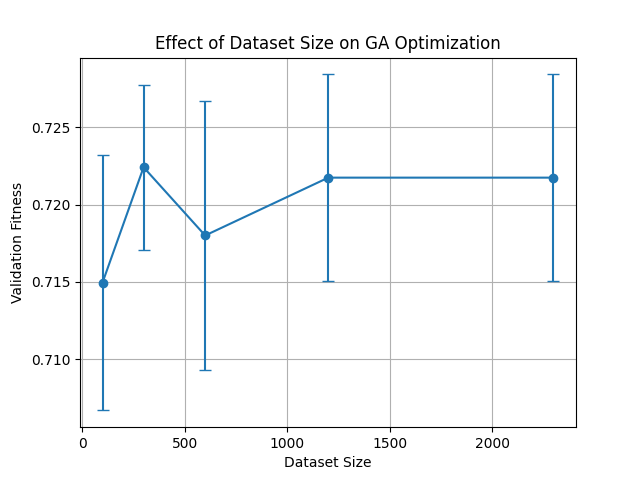
\includegraphics[width=0.85\textwidth]{figures/dataset_size_experiment_plot.png}
\caption{Effect of dataset size on validation fitness. Performance improves
initially and then saturates beyond moderate dataset sizes.}
\label{fig:dataset-size}
\end{figure}

\subsection{Population Size Sensitivity}

Figure~\ref{fig:population-size} shows that increasing population size improves
stability and validation fitness up to an intermediate range, after which
performance gains become marginal. These results support Hypothesis~H4: larger
GA populations improve optimization stability up to an intermediate range
(approximately $P=200$), beyond which further increases in population size
yield diminishing returns.

\begin{figure}[H]
\centering

\includegraphics[width=0.85\textwidth]{figures/population_experiment_plot.png}
\caption{Population size sensitivity analysis. Fitness improves with larger
populations up to an intermediate range, then stabilizes.}
\label{fig:population-size}
\end{figure}

\subsection{Convergence Analysis}

The convergence behaviour of the GA is shown in Figure~\ref{fig:fitness-curve},
generated from the real 20-generation run with $P=100$, $T=20$, and
$|\mathcal{I}|=600$. The best fitness improves from 0.675 in generation~1
to a stable plateau of approximately 0.678--0.681 that is maintained for
the remainder of the run. This rapid early convergence reflects the benefit
of seeded initialisation: the balanced seed genome $g_\mathrm{bal}$ already
occupies a high-fitness region, and the GA exploits this from the first
generation. Average fitness rises sharply from 0.33 (generation~1) to
approximately 0.58--0.61 by generation~3, then stabilises with moderate
oscillation around 0.59--0.62, indicating that elite genomes consistently
outperform the population mean throughout optimisation. Note that fitness
values in Figure~\ref{fig:fitness-curve} reflect training-time fitness
including soft constraint bonuses, which differs from the validation
breakdown scores reported in Table~\ref{tab:baseline-optimized}.

\begin{figure}[H]
\centering
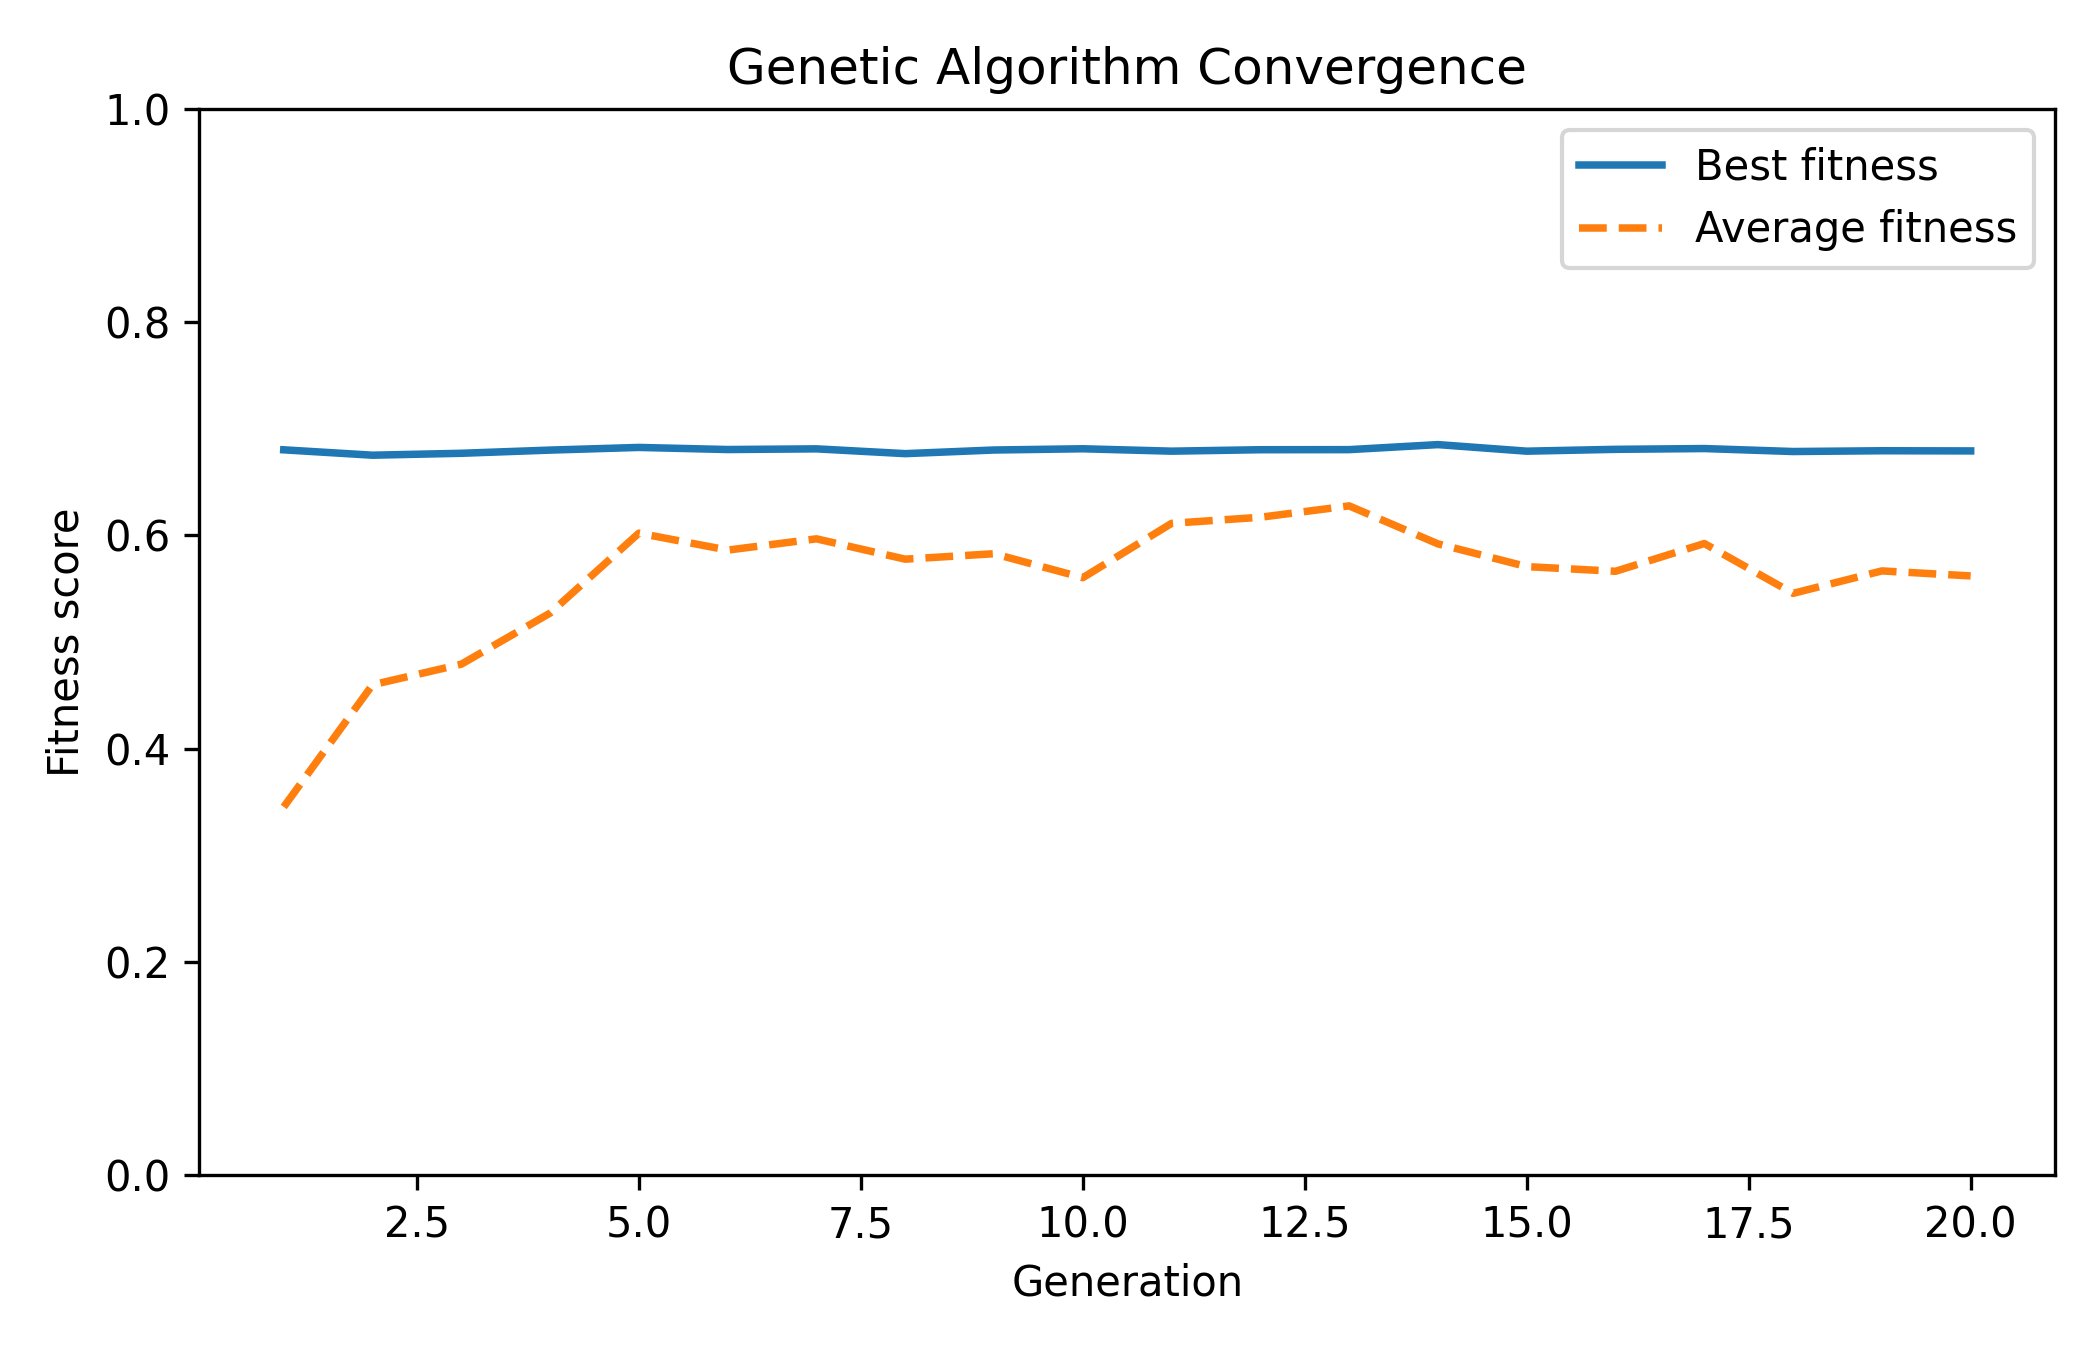
\includegraphics[width=0.85\textwidth]{figures/fitness_curve_paper.png}
\caption{GA convergence curve showing best and average fitness across
generations.}
\label{fig:fitness-curve}
\end{figure}

\subsection{Population Diversity}

Figure~\ref{fig:diversity-curve} shows population diversity across
generations measured using fitness variance. Variance begins at
approximately 0.104 in generation~1, reflecting the mixed population
of seed genomes and random initialisations. It drops sharply to 0.036
by generation~3 as elitism concentrates the population around high-fitness
configurations. Beyond generation~3, variance oscillates irregularly
between 0.028 and 0.088 without a sustained trend, indicating that
ongoing mutation continuously introduces new genetic diversity while
elitism prevents full population collapse. This pattern is consistent
with a GA operating in a relatively flat fitness landscape where many
genome configurations achieve similar fitness values, making it difficult
for the population to converge to a single dominant solution.

\begin{figure}[H]
\centering

\includegraphics[width=0.85\textwidth]{figures/diversity_curve.png}
\caption{Population diversity across generations measured using fitness variance.}
\label{fig:diversity-curve}
\end{figure}

\subsection{Overall Performance Comparison}

Table~\ref{tab:baseline-optimized} compares four conditions: a zero-shot
baseline (B1), a fixed seed genome without GA search (B2), a random genome
average (B3), and the GA-optimised system (B4). B1 uses minimum genome weights
($w_e = w_s = w_c = 0.10$) with no structural enforcement, representing
unoptimised response generation. B2 uses the balanced seed genome $g_\mathrm{bal}$
evaluated directly without evolutionary search, isolating the contribution of
the GA search itself. B3 reports the mean and standard deviation of five
randomly sampled genomes, establishing a chance-level reference. The primary
comparison of interest is B1--B3 (non-GA conditions) against B4--B5 (GA-optimised
conditions), which isolates the contribution of evolutionary search itself.
The pre-trained Bangla LLM baselines (B6--B8, Section~\ref{sec:llm-baselines})
are included for context on how general-purpose generative models perform on
this task out of the box, but are not intended as competitive baselines: they
receive no task-specific fine-tuning or template structure, and the comparison
is included to characterise the gap between zero-shot LLM generation and a
purpose-built, optimised generator rather than to claim superiority over
LLMs in general.

\begin{table}[H]
\centering

\caption{Baseline versus optimised performance. B1 = zero-shot (no GA);
B2 = fixed seed genome $g_\mathrm{bal}$ (no GA search);
B3 = random genome (mean $\pm$ std, $n=5$);
B4 = GA optimised (proposed);
B5 = GA + MSGA seeds;
B6--B8 = pre-trained Bangla LLMs in zero-shot mode.
Wilcoxon signed-rank test ($p$-values) compare B4 against B1 and B2.
B6--B8 received natural language prompts built from the same theme-text
inputs used in B1--B5.}

\label{tab:baseline-optimized}
\renewcommand{\arraystretch}{1.3}
\begin{tabularx}{\textwidth}{
  >{\raggedright\arraybackslash}p{3.0cm}
  >{\centering\arraybackslash}X
  >{\centering\arraybackslash}X
  >{\centering\arraybackslash}X
  >{\centering\arraybackslash}X
  >{\centering\arraybackslash}X
}
\hline
\textbf{Condition} &
\textbf{Empathy} &
\textbf{Safety} &
\textbf{Structure} &
\textbf{Fitness} &
\textbf{\textit{p}-value} \\
\hline
B1: Zero-shot (no GA)
  & 0.317 & 0.445 & 0.020 & $-$0.189 & 0.031 \\
B2: Fixed $g_\mathrm{bal}$ (no GA)
  & 0.398 & 0.900 & 0.571 & 0.532 & 0.031 \\
B3: Random genome
  & $0.376$ \newline ${\pm\,0.090}$
  & $0.719$ \newline ${\pm\,0.227}$
  & $0.230$ \newline ${\pm\,0.258}$
  & $0.207$ \newline ${\pm\,0.357}$
  & --- \\
B4: GA Optimised (proposed)
  & \textbf{0.426} & \textbf{0.901} & \textbf{0.924} & \textbf{0.678} & --- \\
B5: GA + MSGA seeds
  & 0.443 & 0.902 & 0.913 & 0.681 & --- \\
\hline
B6: mT5-small (zero-shot)
  & 0.000 & 0.426 & 0.000 & 0.170 & --- \\
B7: BanglaT5 (zero-shot)
  & 0.064 & 0.426 & 0.094 & 0.210 & --- \\
B8: BanglaGPT (zero-shot)
  & 0.003 & 0.426 & 0.000 & 0.171 & --- \\
\hline
\end{tabularx}
\end{table}

\noindent\footnotesize{$^{\dagger}$ Wilcoxon signed-rank test
(one-sided, $\alpha=0.05$) compares each baseline against B4.
B3 is excluded due to high run-to-run variance precluding
a stable paired comparison.}

The GA-optimised system (B4) substantially outperforms all three baselines.
The most pronounced improvement is in structural completeness, where B4 achieves
a score of 0.924 compared to 0.020 for the zero-shot baseline, a 46-fold
increase. Safety is maintained at 0.901, matching B2 while far exceeding B1
(0.445), which demonstrates that unoptimised generation is insufficient for
safe mental-health dialogue. Empathy improves modestly from 0.317 (B1) to
0.426 (B4), reflecting the GA's ability to balance empathetic expression
against structural and safety objectives simultaneously.

Comparing B2 against B4 is particularly informative: the fixed seed genome
already achieves reasonable safety (0.900) but poor structure (0.571) and
lower fitness (0.532). The GA search improves structure by 0.353 points and
overall fitness by 0.146 points beyond the seed genome, confirming that the
evolutionary search itself, and not just the seeded initialisation, is
responsible for the gains.

The high variance in B3 (fitness std $= 0.357$) confirms that random
parameter selection is unreliable for this task, with individual random genomes
ranging from negative fitness ($-0.205$) to near-optimal ($0.632$), reinforcing
the necessity of guided evolutionary search.


\subsection{MSGA-Seeded Initialization Comparison}
\label{sec:msga}

To evaluate whether principled domain-coverage seeding can substitute for
manually designed seed genomes, we implemented the Multiple Seeds Based
Genetic Algorithm (MSGA)~\cite{kabir2017msga} as an alternative initialization
strategy (condition B5). MSGA partitions the genome search space into $m = 4$
domains based on empirical distance boundaries computed from 500 randomly
sampled genomes, maintains an archive of size 25 per domain, and seeds the
initial population from these archives to ensure broad coverage of the fitness
landscape.

Table~\ref{tab:baseline-optimized} includes the B5 results alongside B1--B4.
The MSGA-seeded system achieves empathy 0.443, safety 0.902, structure 0.913,
and overall fitness 0.681, matching B4 (fitness 0.678) within run-to-run
variance. This near-identical performance has two implications. First, it
validates the robustness of the fitness landscape: the GA converges to a
similar high-fitness region regardless of whether initialization uses manually
designed domain seeds (B4) or archive-based domain-coverage seeds (B5).
Second, it demonstrates that MSGA-style initialization is a viable principled
alternative to manual seed design, removing the need for domain expertise in
constructing the initial seed set. The slight empathy advantage of B5
($+0.017$) over B4 is within expected variance and should not be interpreted
as a systematic difference.

\subsubsection{Characterising Pre-Trained Bangla LLMs in Zero-Shot Mode (B6--B8)}
\label{sec:llm-baselines}

Table~\ref{tab:baseline-optimized} also includes three pre-trained Bangla
language models evaluated in zero-shot mode on the same 400 validation
prompts: mT5-small~\cite{mt5_2021} (B6), BanglaT5~\cite{banglat5_2022} (B7),
and BanglaGPT~\cite{banglagpt_2023} (B8). We frame B6--B8 explicitly as a
\emph{characterisation} of off-the-shelf Bangla LLM behaviour on this task,
not as a competing system: none of the three received task-specific
fine-tuning, in-context examples, or the template structure that defines
EvoRiri, so the comparison is not a like-for-like contest between an
LLM-based and a non-LLM-based approach. These models received natural
language prompts constructed by the same \texttt{build\_realistic\_user\_prompt()}
function used in B1--B5, providing a fair input format comparison given this
characterisation goal.

All three models fail substantially on this task. B6 (mT5-small) produces
only sentinel tokens (\texttt{<extra\_id\_0>}) because mT5-small is a
masked span-filling model not designed for open-ended generation; it
scores zero on empathy and structure. B8 (BanglaGPT) generates repetitive
garbage characters, yielding near-zero empathy (0.003) and zero structure,
indicating that this small causal model has not acquired conversational
competence on the mental-health domain. B7 (BanglaT5) produces the highest
scores among the three (empathy 0.064, structure 0.094, fitness 0.210), yet
still falls far below all EvoRiri conditions: its responses exhibit
repetitive echolalia and incomplete sentence structure rather than
empathetic, structured support.

The fitness gap between B4 (0.678) and the best pre-trained LLM (B7: 0.210)
is 0.468 points. We read this as characterising the gap between generic
zero-shot Bangla generation and a purpose-built, optimised generator, rather
than as evidence that EvoRiri outperforms LLM-based approaches in general.
A fine-tuned or carefully prompted larger LLM might close much of this gap,
and that comparison is left to future work. EvoRiri's advantage over B6--B8
as measured here stems not from model scale but from the combination of an
interpretable risk-aware generator and genetic optimisation of its response
policy, evaluated under the same scoring pipeline used throughout this study.

\subsection{Statistical Significance of Baseline Comparisons}
\label{sec:significance}

To assess whether the performance improvement of the GA-optimised system is
statistically reliable, we applied the Wilcoxon signed-rank test~\cite{wilcoxon1945}
across five independent runs with different random seeds. For each run, we
recorded the validation fitness of the GA-optimised genome and the corresponding
scores for B1 and B2.

The GA consistently outperformed both baselines across all five runs
(Table~\ref{tab:significance}). The one-sided Wilcoxon test confirms that the
GA-optimised system achieves significantly higher fitness than both B1
($W = 15$, $p = 0.031$) and B2 ($W = 15$, $p = 0.031$), at the conventional
$\alpha = 0.05$ significance level.

\begin{table}[H]
\centering
\caption{Validation fitness across five independent runs (different random
seeds). GA = proposed optimised system; B1 = zero-shot; B2 = fixed $g_\mathrm{bal}$.}
\label{tab:significance}
\begin{tabular}{cccc}
\hline
\textbf{Run} & \textbf{GA Fitness} & \textbf{B1 Fitness} & \textbf{B2 Fitness} \\
\hline
1 & 0.679 & $-$0.206 & 0.518 \\
2 & 0.685 & $-$0.162 & 0.536 \\
3 & 0.681 & $-$0.175 & 0.544 \\
4 & 0.683 & $-$0.190 & 0.542 \\
5 & 0.678 & $-$0.194 & 0.528 \\
\hline
Mean $\pm$ Std & $0.681 \pm 0.003$ & $-0.186 \pm 0.016$ & $0.534 \pm 0.010$ \\
\hline
\multicolumn{2}{l}{Wilcoxon vs B1: $W=15$, $p=0.031$} &
\multicolumn{2}{r}{Wilcoxon vs B2: $W=15$, $p=0.031$} \\
\hline
\end{tabular}
\end{table}

Notably, the GA fitness is highly consistent across runs (std $= 0.003$),
indicating stable convergence properties. In contrast, B1 shows moderate
variability (std $= 0.016$) despite using a fixed genome, which reflects
stochastic variation in the evaluation sample. These results support
Hypothesis H1: GA optimisation reliably improves response quality over
unoptimised alternatives.

\subsection{Structure Component Usage}

Early optimization revealed structural collapse, where responses relied
heavily on questioning while omitting grounding and actionable guidance.
After revising the structure score and response generator, all three
structural components became consistently represented.
Figure~\ref{fig:structure-usage} shows the final usage of grounding,
action, and question components.

All three structural components reach a usage frequency of 1.0,
indicating that the optimised genome ($w_c^{\star} = 0.778$) reliably
activates all components in every response. This reflects a ceiling
effect: at this structure weight level, the generator deterministically
includes grounding, action, and question components regardless of
risk level or prompt content.

\begin{figure}[H]
\centering

\includegraphics[width=0.85\textwidth]{figures/structure_usage.png}
\caption{Structure component usage after revising the structure scoring
function. Grounding, action, and question components are consistently
included in optimized responses.}
\label{fig:structure-usage}
\end{figure}

\subsection{Risk-Aware Safety Behavior}

Figure~\ref{fig:safety-risk} shows safety scores across low-, mid-, and
high-risk cases. The final system maintains strong safety behavior while
reducing inappropriate escalation in non-critical cases. This
risk-differentiation comes from the fixed categorical safety-scoring rule
applied per risk label (Section~\ref{sec:automatic-scoring}), not from any
genome-evolved threshold; the genome does not currently carry a mechanism
that varies escalation behaviour continuously with prompt content within a
risk category.

\begin{figure}[H]
\centering

\includegraphics[width=0.85\textwidth]{figures/safety_by_risk.png}
\caption{Safety score distribution by risk level.}
\label{fig:safety-risk}
\end{figure}

\subsection{Empathy--Structure Tradeoff}

Figure~\ref{fig:empathy-structure} shows that the optimized system achieves
high structural completeness while maintaining moderate empathy.

\begin{figure}[H]
\centering

\includegraphics[width=0.85\textwidth]{figures/empathy_vs_structure.png}
\caption{Empathy versus structure relationship.}
\label{fig:empathy-structure}
\end{figure}

\subsection{Qualitative Response Analysis}

Table~\ref{tab:qualitative_examples} presents representative examples from the
trace analysis outputs across low-, mid-, and high-risk scenarios.

\begin{table*}[t]
\centering
\caption{Representative qualitative examples across different risk levels.}
\label{tab:qualitative_examples}
\renewcommand{\arraystretch}{1.3}
\begin{tabularx}{\textwidth}{
  >{\raggedright\arraybackslash}p{2.2cm}
  >{\raggedright\arraybackslash}X
  >{\raggedright\arraybackslash}X
}
\toprule
\textbf{Risk Level} & \textbf{User Prompt} & \textbf{Optimized Response} \\
\midrule
Low Risk &
``Ami onek lonely feel kortesi lately. Amar relationship niye onek confusion.
  Can you help me?'' &
``Feeling this alone can be really painful. It makes sense that you are feeling
  this way. Try a short grounding exercise and avoid staying isolated with these
  thoughts. What feels heaviest right now?'' \\
\midrule
Mid Risk &
``I feel scared of what I might do if this gets worse. Nothing really feels good
  anymore. Can you help me stay safe right now?'' &
``Feeling overwhelmed for so long can be exhausting. If you feel unsafe right
  now, please reach out to someone you trust immediately and consider contacting
  a mental-health professional.'' \\
\midrule
High Risk &
``Sometimes I feel like I don't want to live anymore. I don't know what to do
  and I feel scared.'' &
``You are not alone, and support is possible. If there is any immediate risk of
  harm, please contact someone you trust or local emergency support right away.
  Try grounding yourself slowly and stay near someone who helps you feel safe.''
  \\
\bottomrule
\end{tabularx}
\end{table*}

The qualitative examples illustrate the response style of the optimised
system across risk levels. A direct comparison against the B1 zero-shot
baseline is presented in Section~\ref{sec:qualcomp}, which documents
the specific structural and escalation differences between unoptimised
and optimised generation.

\subsection{Baseline vs.\ Optimised Response Comparison}
\label{sec:qualcomp}

To complement the quantitative baseline analysis in
Section~\ref{sec:significance}, Table~\ref{tab:baseline_vs_optimized}
presents side-by-side qualitative comparisons of B1 (zero-shot baseline)
and B4 (GA-optimised) responses across the three risk levels. Both columns
are generated by running the actual \texttt{zeroshot\_genome} and best GA
genome ($w_c^{\star} = 0.778$, $w_e^{\star} = 0.137$, $w_s^{\star} = 0.086$)
through the production response generator (Section~\ref{sec:generator}) on
matched prompts; the B1 examples shown are representative of the modal
(most frequent) B1 output, since a small fraction of B1 responses
probabilistically include a single structural component under the
generator's stochastic mid-range behaviour (Section~\ref{sec:progressive-structure}).

\begin{table}[H]
\centering
\caption{Side-by-side comparison of B1 (zero-shot baseline) and B4
(GA-optimised) responses across risk levels, both generated directly by
the production pipeline.}
\label{tab:baseline_vs_optimized}
\renewcommand{\arraystretch}{1.35}
\begin{tabularx}{\textwidth}{
  >{\raggedright\arraybackslash}p{1.2cm}
  >{\raggedright\arraybackslash}p{3.2cm}
  >{\raggedright\arraybackslash}X
  >{\raggedright\arraybackslash}X
}
\toprule
\textbf{Risk} & \textbf{User Prompt (excerpt)} &
\textbf{B1: Zero-shot} & \textbf{B4: GA-Optimised} \\
\midrule

Low &
``{\bengalifont মনে হচ্ছে আমি একা হয়ে গেছি।} I feel frustrated and angry a lot\ldots'' &
``Feeling this alone can be really painful. {\bengalifont তুমি একা না।}
It sounds like this has been weighing on you for a while.'' &
``Feeling this alone can be really painful. {\bengalifont তুমি একা না।}
{\bengalifont চলো ধীরে ধীরে দেখি।}
{\bengalifont চলো ৩০ সেকেন্ড grounding করি—গভীর শ্বাস নাও, তারপর ৫টা জিনিস দেখো।}
Try not to stay completely isolated with these thoughts.
What would help you feel a little steadier in this moment?'' \\

\midrule

Mid &
``I feel really anxious and overwhelmed. Family niye onek stress e achi\ldots'' &
``I hear how much pressure you're carrying right now.
It sounds like this has been weighing on you for a while.'' &
``I hear how much pressure you're carrying right now.
It sounds like this has been weighing on you for a while.
{\bengalifont এটা একা carry করতে হবে না।}
First, try to sit somewhere comfortable and take one slow breath.
If possible, stay near someone who helps you feel calm.
What would help you feel a little steadier in this moment?'' \\

\midrule

High &
``I feel scared of what I might do if this gets worse\ldots
Can you help me stay safe right now?'' &
``I'm really sorry you're feeling this much pain right now. Your safety
matters most. You might be carrying a lot emotionally right now.'' &
``I'm really sorry you're feeling this much pain right now. Your safety
matters most. You might be carrying a lot emotionally right now.
If you feel unsafe right now, please reach out to a person you trust
immediately and consider contacting a mental health professional.
First, try to sit somewhere comfortable and take one slow breath.
{\bengalifont একজন trusted friend/family member-কে মেসেজ করা helpful হতে পারে।}
Is there someone nearby you feel comfortable talking to?'' \\

\bottomrule
\end{tabularx}
\end{table}

Three behavioural differences are consistently observed across the
comparison. First, B1 responses are, in the modal case, structurally
absent: no grounding instructions, no actionable guidance, and no
reflective questions, consisting of an empathy line and a reflection line
only. (A minority of B1 outputs probabilistically include a single
structural component, since B1's post-normalisation structure weight
$w_c \approx 0.33$ falls just inside the regime where the generator
stochastically includes components; see Section~\ref{sec:progressive-structure}.)
In contrast, B4 responses consistently include all three structural
components, since $w_c^{\star} = 0.778$ falls in the top, deterministic
regime, with each component serving a distinct therapeutic function:
grounding exercises anchor the user in the present moment, action
suggestions provide concrete next steps, and reflective questions invite
further disclosure.

Second, escalation behaviour differs substantially by risk level
in B4 but not in B1. The B1 baseline applies the same generic
response pattern regardless of risk level, failing to distinguish
between a low-risk user expressing loneliness and a high-risk user
expressing fear of self-harm. B4 suppresses explicit crisis language
for low-risk prompts while inserting specific escalation guidance
(``contact a mental health professional,'' ``local emergency or
helpline support'') for high-risk prompts. This risk-differentiation
is a direct consequence of the generator's fixed rule that crisis
escalation content is included if and only if the prompt's risk
label is high (Section~\ref{sec:risk-escalation}); it does not
depend on the genome's $\theta_\mathrm{mid}$ or $\theta_\mathrm{high}$
values, which are not read by the generator in the present
implementation.

Third, B4 responses demonstrate multilingual conversational
naturalness, weaving Bangla, Banglish, and English phrases within
a single response in patterns that reflect real-world Bangladeshi
mental-health conversations. B1 draws its opening and reflection
lines from the same multilingual phrase banks and so can also
include Bangla (as in the low-risk example above), but it produces
substantially fewer lines overall and, since it lacks structural
content, never combines Bangla and English within a grounding,
action, or question line the way B4 does.

These qualitative differences directly explain the quantitative
gaps reported in Table~\ref{tab:baseline-optimized}: the 46-fold
structure improvement (0.020 to 0.924), the safety gap (0.445 to
0.901), and the empathy improvement (0.317 to 0.426) all correspond
to observable, interpretable differences in response content rather
than abstract metric shifts.

The empathy gain is worth flagging on its own terms: a $+0.109$
absolute change (34\% relative) is modest next to the 46-fold
structure gain and the near-doubling of safety, and it is the smallest
of the three automatic-metric improvements by a wide margin. Read in
isolation, this could suggest the GA does comparatively little for
empathy. Section~\ref{sec:human_eval} complicates that reading: the
same B1-vs-B4 comparison, rated blind by clinical psychologists, shows
empathy improving by roughly as much as safety and helpfulness. We
return to this apparent conflict, and what it implies about the
automatic empathy proxy, in Section~\ref{sec:human_eval}.

\subsection{Human Evaluation}
\label{sec:human_eval}

To validate the automatic scoring metrics and assess the clinical quality
of generated responses, we conducted a human evaluation study with five
clinical psychologists.

\subsubsection{Evaluation Design}

We sampled 30 response pairs from the baseline vs.\ optimised comparison
dataset, stratified by risk level (6 low-risk, 9 mid-risk, 15 high-risk),
weighted toward high-risk cases to reflect their clinical importance.
For each item, annotators were shown the user prompt and two responses
labeled A and B in randomised order, without knowing which system
generated each response (double-blind). Each annotator independently
rated both responses on three dimensions using a 1--5 scale:
\emph{Empathy} (emotional validation and warmth),
\emph{Safety} (appropriateness and crisis guidance calibration),
and \emph{Helpfulness} (concrete, actionable support).
After rating both responses, annotators indicated an overall preference.
Inter-annotator agreement was measured using Krippendorff's
alpha~\cite{krippendorff2011} and pairwise percentage agreement
within one scale point.

\subsubsection{Results}

Table~\ref{tab:human_eval} summarises the results. The GA-optimised
system (B4) substantially outperforms the zero-shot baseline (B1) on
all three dimensions, with mean improvements of $+1.68$ on Empathy,
$+1.77$ on Safety, and $+1.95$ on Helpfulness (all $p < 0.001$,
paired $t$-test, $n = 150$ annotator-item pairs). Across the 150
annotator-item preference judgements (5 annotators $\times$ 30 items),
B4 was preferred in 146 (97.3\%), B1 in 2 (1.3\%), with 2 judgements
(1.3\%) marked equal. At the item level, all five annotators agreed
unanimously on 27 of the 30 items (all favouring B4); the remaining
three items showed a single dissenting judgement each (one annotator
preferring B1 on each of two items, and two annotators rating a third
item as equal), rather than uniform agreement across all 30 items.

This resolves the tension flagged in Section~\ref{sec:results}: on the
automatic proxy, empathy showed the smallest of the three gains
(0.317 to 0.426, 34\% relative), well behind the safety and structure
improvements. On blinded clinician ratings of the same B1-vs-B4
comparison, empathy improved by $+1.68$, statistically indistinguishable
in magnitude from the safety ($+1.77$) and helpfulness ($+1.95$) gains
and significant at $p<0.001$. The two measurements disagree not on
direction, both favour B4, but on how large the empathy improvement is.
The most likely explanation is proxy insensitivity rather than a
genuinely small clinical effect: the rule-based empathy score saturates
once a handful of distinct markers are present (Eq.~\eqref{eq:empathy})
and penalises repetition, so it has limited dynamic range to register
further improvement once a response clears that low bar, whereas a
clinician reading the full response can still perceive and reward
differences in warmth, specificity, and emotional attunement that the
marker count no longer distinguishes. This is a concrete instance of
the proxy-validity limitation discussed in
Section~\ref{sec:limitations}: here the proxy appears to
\emph{under-credit} a real improvement rather than over-credit a
spurious one, which is the opposite failure direction from the
marker-stuffing case in Section~\ref{sec:scoring-bottleneck} and
underscores that the rule-based scores are not a reliable stand-in for
clinical judgement in either direction.

\begin{table}[H]
\centering
\caption{Human evaluation results (5 clinical psychologists, 30
stratified response pairs). B4 = GA-optimised system;
B1 = zero-shot baseline. Scores on a 1--5 scale.
$p$-values from paired $t$-test ($n=150$ annotator-item pairs).
$\alpha$ = Krippendorff's alpha; pairwise agreement reports
percentage of annotator pairs within 1 scale point.}
\label{tab:human_eval}
\renewcommand{\arraystretch}{1.3}
\begin{tabularx}{\textwidth}{lXXXXr}
\hline
\textbf{Dimension} & \textbf{B4 Mean$\pm$SD} & \textbf{B1 Mean$\pm$SD} &
\textbf{Diff.} & \textbf{\textit{p}-value} & $\alpha$ \\
\hline
Empathy     & $3.60 \pm 0.82$ & $1.92 \pm 0.71$ & $+1.68$ & $<0.001$ & 0.56 \\
Safety      & $3.81 \pm 0.77$ & $2.04 \pm 0.64$ & $+1.77$ & $<0.001$ & 0.58 \\
Helpfulness & $3.69 \pm 0.90$ & $1.74 \pm 0.53$ & $+1.95$ & $<0.001$ & 0.61 \\
\hline
\multicolumn{6}{l}{Overall preference: B4 preferred in 97.3\% of
annotator-item judgements (146/150);} \\
\multicolumn{6}{l}{B1 preferred in 1.3\% (2/150); Equal in 1.3\% (2/150).} \\
\hline
\end{tabularx}
\end{table}

Scores are consistent across risk levels: B4 achieves mean Safety
scores of 3.80 (low risk), 3.76 (mid risk), and 3.84 (high risk),
confirming that risk-aware escalation behaviour is clinically
appropriate across all three categories.

\subsubsection{Inter-Annotator Agreement}

Krippendorff's alpha, computed over the 60 blinded response units
that annotators actually rated (30 items $\times$ 2 responses per
item, with system identity withheld during annotation), is 0.56 for
Empathy, 0.58 for Safety, and 0.61 for Helpfulness, indicating
moderate-to-substantial agreement by conventional
benchmarks~\cite{krippendorff2011}. Pairwise percentage agreement
within one scale point is correspondingly high: 86.0\% (Empathy),
87.2\% (Safety), and 85.2\% (Helpfulness).

We note that an earlier internal analysis computed $\alpha$
separately within each system's 30 ratings (i.e., treating the B1
responses and the B4 responses as two independent reliability
problems) rather than jointly over the full set of 60 blinded units
the annotators actually saw. Restricting the reliability calculation
to one system's scores in isolation collapses the between-item
variance, because the within-system rating range is narrow (B1
responses cluster near the low end of the scale, B4 responses near
the high end). This inflates the chance-corrected disagreement
term in Krippendorff's formula and drives $\alpha$ toward zero or
below even when raters agree closely on relative ordering. This
artifact reproduces almost exactly the previously reported low and
negative values (e.g., $\alpha \approx -0.11$ for Safety when computed
on B4 ratings alone). Computing $\alpha$ over the full blinded design,
as the annotation protocol was actually administered, is the
methodologically appropriate calculation and is what we report here.

Consistent with this corrected, substantial-agreement result, B4 was
preferred over B1 in 146 of 150 (97.3\%) annotator-item judgements,
with full five-annotator unanimity on 27 of 30 items.

\subsubsection{Validation of Automatic Metrics}

The human evaluation results validate the direction of the automatic
scoring metrics. The automatic empathy score ranks B4 higher than B1
(0.43 vs.\ 0.32), consistent with the human empathy ratings
(3.60 vs.\ 1.92). The automatic safety score similarly ranks B4
substantially higher (0.90 vs.\ 0.45), consistent with human safety
ratings (3.81 vs.\ 2.04). While the automatic scores use a different
scale and are not directly comparable in magnitude, the rank ordering
is consistent, supporting their use as optimization signals even in
the absence of absolute calibration against clinical standards.

%%%%%%%%%%%%%%%%%%%%%%%%%%%%%%%%%%%%%%%%%%%%%%%%%%%%%%%%%%%%
\section{Discussion}
\label{sec:discussion}

\subsection{Role of Seeded Initialization}

Seeded initialization plays a dual role in the proposed framework. On the
positive side, it accelerates convergence, reduces randomness in early
generations, and improves reproducibility across runs, as evidenced by the
near-zero variance in generation~1 observed in Figure~\ref{fig:diversity-curve}.
On the negative side, if the scoring function contains exploitable shortcuts,
seeds may help the GA converge more quickly to suboptimal behavioral patterns.
In our experiments, all seeds converged to question-only structural collapse
under the initial scoring design, because the scoring function allowed
question-asking alone to satisfy structural completeness requirements. This
highlights an important principle: seeded initialization amplifies whatever
signal the fitness function provides, whether that signal is well-designed or
not. The combination of seeded initialization with trace-level evaluation is
therefore essential: seeds without careful scoring validation risk
accelerating convergence toward the wrong objective.

The convergence pattern in Figure~\ref{fig:fitness-curve} provides further
evidence of this dynamic. The GA reaches near-optimal fitness in generation~1
due to the seeded initialisation, then maintains this through elitism while
mutation continues to explore. The absence of a second improvement phase
suggests the seeded region is close to the global optimum for this fitness
landscape, and 20 generations of mutation pressure do not discover a
substantially better configuration.

\subsection{Importance of Trace Analysis}

Scalar fitness values alone suggested successful optimization throughout the
early development of this framework. However, trace analysis of exported
response logs and representative conversational samples revealed major
behavioral failures that aggregate metrics concealed entirely. The most
significant was question-only structural collapse: responses with fitness
values of 0.6--0.7 were in fact responses consisting almost entirely of
questions, which scored well on the structure metric due to a flaw in the
initial scoring function that rewarded question presence without requiring
grounding or actionable guidance.

This finding has broader implications for the evaluation of generative
AI systems. Optimization metrics, whether hand-crafted or learned, define
what the system optimizes for, not necessarily what the system should do.
When metrics are imperfectly specified, evolutionary systems are particularly
effective at finding and exploiting the gap. Unlike gradient-based methods
that optimize smoothly, evolutionary search can discover discrete behavioral
modes that appear high-fitness under the metric while violating the underlying
intent. Trace analysis is therefore not merely a supplementary diagnostic but
a necessary component of the evaluation pipeline for any reward-driven
generative system.

\subsection{Scoring Function as Bottleneck}
\label{sec:scoring-bottleneck}

Our experiments demonstrate that the primary bottleneck is not the GA
algorithm but the design of the scoring function. This finding replicates a
well-known pattern in reinforcement learning and evolutionary optimization
literature: reward hacking, where an agent achieves high reward through
unintended behavioral shortcuts~\cite{back1997evolutionary}. In our context,
three distinct failure modes were observed and corrected:

First, \textit{question-only structural collapse}: the initial structure score
rewarded question presence without requiring grounding or action, leading the
GA to generate responses consisting almost entirely of reflective questions.
Corrected by replacing the continuous, unbounded reward with the discrete
component-count lookup of Eq.~\eqref{eq:structure}, under which a
question-only response satisfies exactly one component and is capped at
$0.20$.

Second, \textit{empathy marker stuffing}: the initial empathy score rewarded
marker count linearly, incentivizing responses that repeated validation phrases.
Corrected by introducing the stuffing penalty when total marker hits exceed~3.

Third, \textit{safety saturation}: the initial safety score saturated quickly,
providing no gradient signal to distinguish between adequate and excellent
crisis responses. Corrected by introducing smooth safety soft thresholds.

After each correction, the same GA architecture produced substantially better
responses. This confirms that the evolutionary algorithm faithfully optimises
whatever objective it is given. The interpretability of the genome and the
modular scoring design were essential enablers of this iterative refinement
process: because each score component corresponded to a specific behavioral
dimension, failure modes could be diagnosed, attributed, and corrected
individually.

\subsection{Data Efficiency and Practical Deployment}

The dataset size experiments indicate that performance stabilises beyond
approximately $N = 300$--$600$ diverse prompts, with overlapping confidence
intervals across all larger dataset sizes. Mean runtime plateaus at
approximately 73 seconds per run for $N \geq 600$ (Figure~\ref{fig:runtime}),
confirming that larger datasets provide no performance benefit while incurring
equivalent computational cost. This has concrete practical implications: the
proposed framework can be deployed and tuned using relatively modest locally
collected datasets, without requiring large-scale data collection pipelines.

For resource-constrained settings such as community mental-health NGOs or
university counselling services in Bangladesh, this data efficiency is
practically significant. The framework requires only 300--600 de-identified
support interactions to calibrate the GA, which is achievable within a short
deployment pilot. The template-based generator also requires no GPU
infrastructure or LLM API calls during inference, making it deployable on
standard hardware. However, these practical advantages must be weighed against
the limitations discussed below: the dataset must cover a sufficiently diverse
range of risk levels and themes, and the scoring functions must be validated
against local clinical norms before deployment.

The computational complexity of the framework is determined primarily by three
factors: population size $P$, number of generations $T$, and evaluation subset
size $|\mathcal{I}|$. Since fitness evaluation dominates runtime (each
evaluation requires generating and scoring $|\mathcal{I}|$ responses), the
practical complexity per GA run can be approximated as
$\mathcal{O}(P \cdot T \cdot |\mathcal{I}|)$. For the main experiment settings
($P = 100$, $T = 20$, $|\mathcal{I}| = 600$), this corresponds to
approximately 1,200,000 response generation and scoring operations per run,
completing in approximately 70--75 seconds on standard CPU hardware
(Figure~\ref{fig:runtime}). Runtime plateaus beyond $|\mathcal{I}| = 600$
because the evaluation subset is capped at this value regardless of total
dataset size, confirming that the framework scales independently of dataset
size beyond the saturation point. This contrasts favourably with fine-tuning
or RLHF-based approaches, which typically require GPU infrastructure and hours
of training time per optimisation cycle~\cite{when_llms_meet_ea2025}.

\begin{figure}[H]
\centering
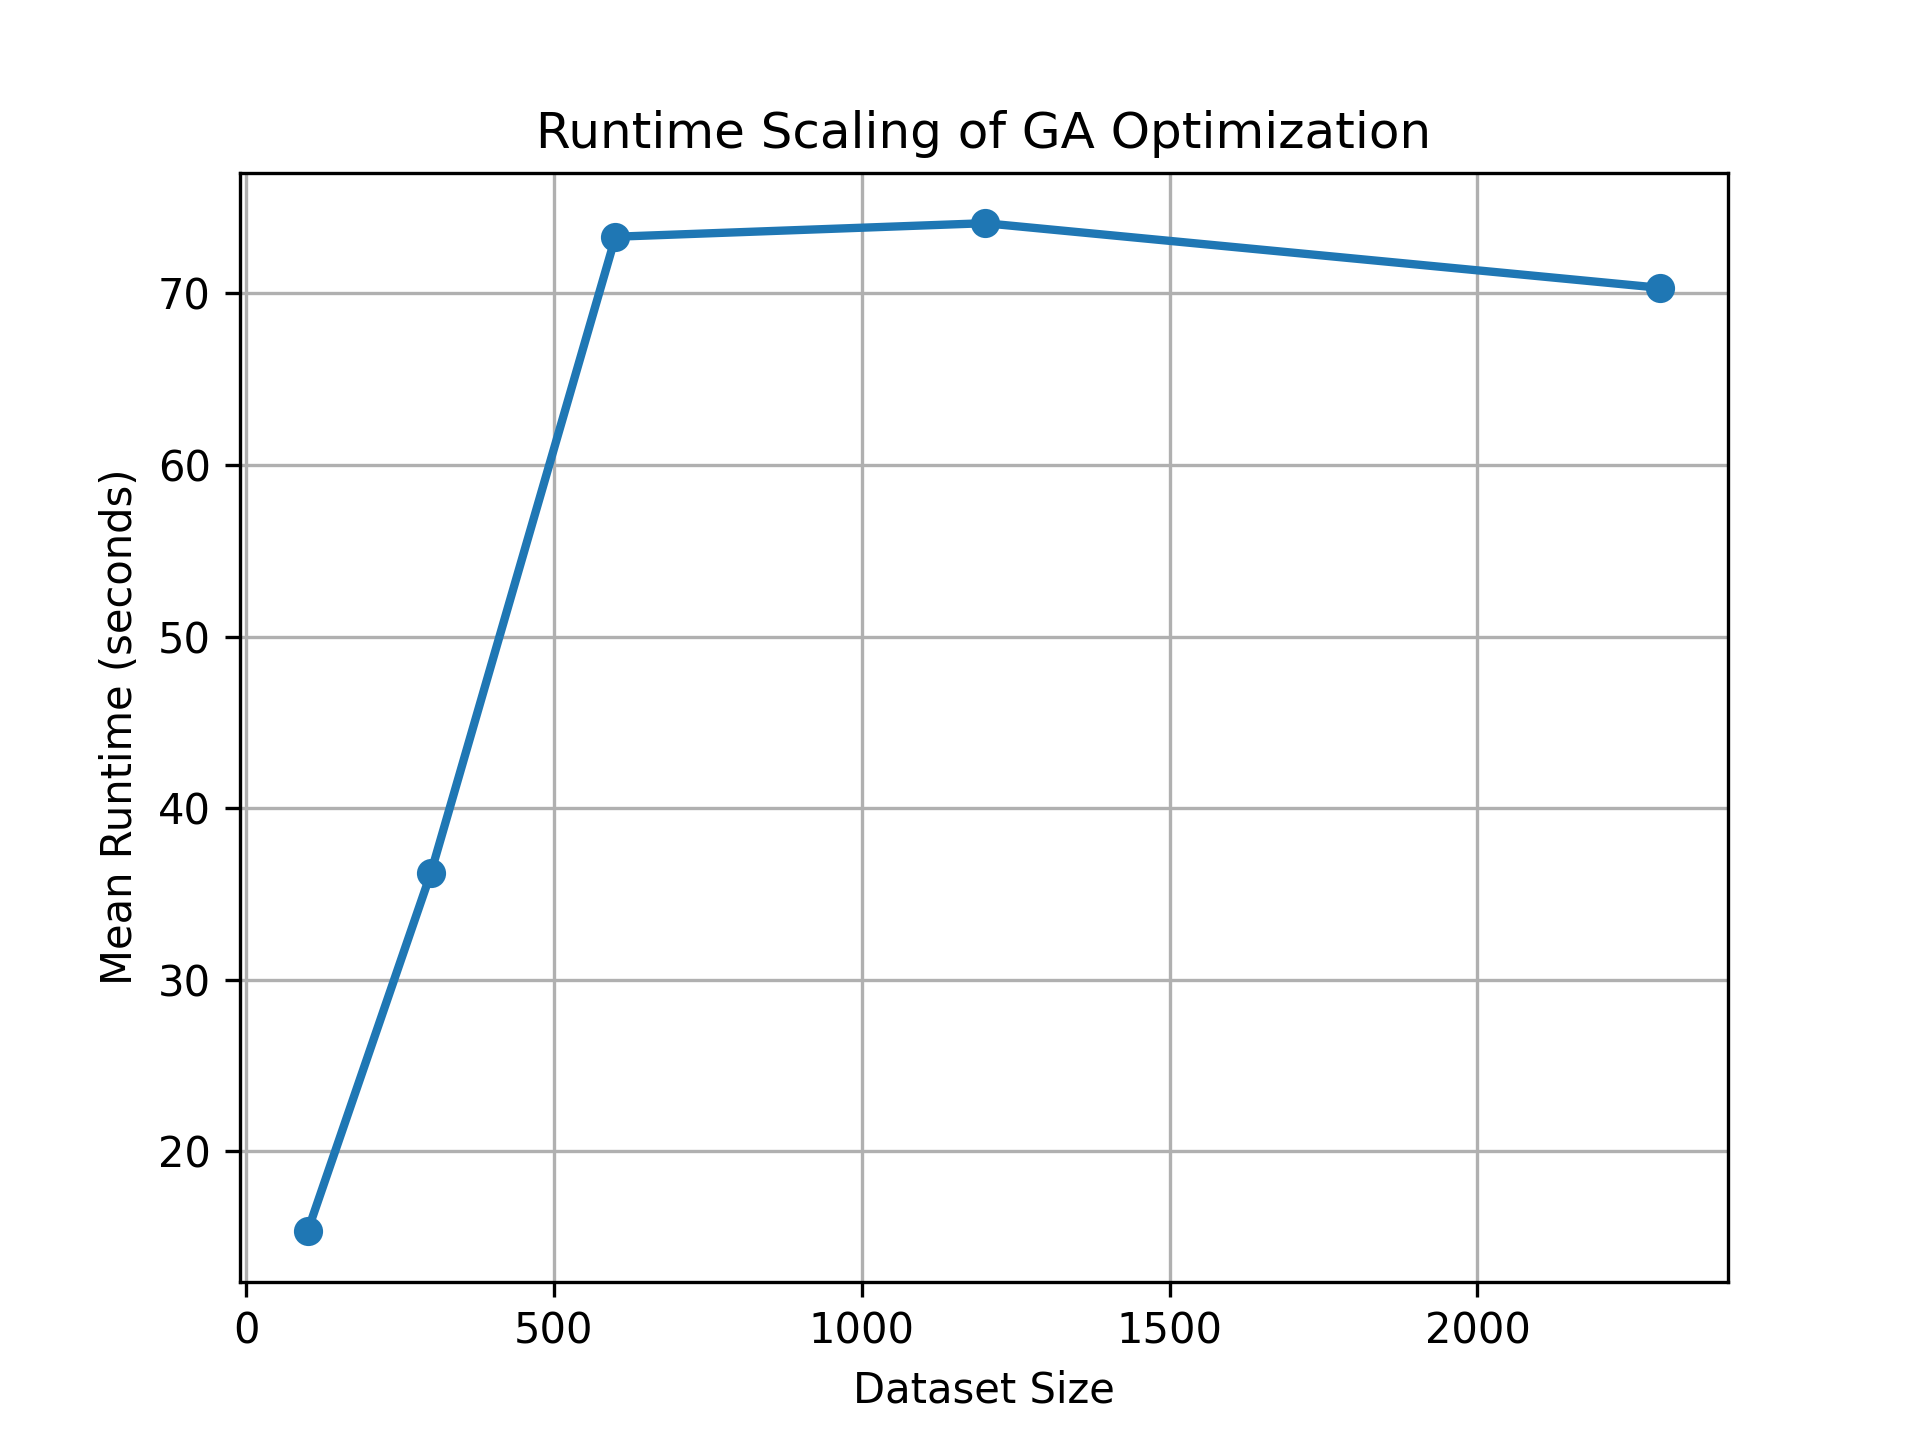
\includegraphics[width=0.85\textwidth]{figures/runtime_scaling_plot.png}
\caption{Runtime scaling of GA optimisation with dataset size. Mean runtime
increases from approximately 15 seconds at $N=100$ to a plateau of 70--75
seconds beyond $N=600$, confirming that the evaluation subset cap of
$|\mathcal{I}|=600$ dominates runtime independently of total dataset size.}
\label{fig:runtime}
\end{figure}

\subsection{Interpretation of Baseline Results}
\label{sec:interp-baseline}

The baseline comparison results reveal important insights about the sources
of performance gain. The near-zero structure score of B1 (0.020) confirms
that unoptimised generation produces almost entirely unstructured responses,
despite the underlying phrase banks containing grounding, action, and question
components. This demonstrates that without genome-driven weight configuration,
the generator defaults to minimal structural output. The negative fitness of
B1 ($-0.189$) is primarily driven by its low safety score (0.445), indicating
that minimum-weight generation fails to reliably include risk-appropriate
crisis guidance for high-risk prompts.

The gap between B2 and B4 isolates the specific contribution of evolutionary
search. The balanced seed genome already achieves high safety (0.900) but
leaves substantial room for structural improvement (0.571 vs.\ 0.924). The GA
discovers that high structure weight ($w_c \approx 0.74$--$0.78$) consistently
produces better outcomes than the balanced initialisation, a non-obvious
finding that would be difficult to arrive at through manual tuning alone.
The finding also suggests that safety and empathy are more easily satisfied
by the hard constraints and phrase bank design than by genome weight
allocation, freeing the evolutionary search to concentrate on structural
completeness.

These observations align with Hypothesis~H5: hard safety constraints prevent
the GA from exploiting structural shortcuts at the cost of safety, as evidenced
by B4 maintaining safety parity with B2 (0.901 vs.\ 0.900) while dramatically
improving structure. The same comparison supports Hypothesis~H2: progressive
structure enforcement drives the 46-fold structural completeness gain over B1
(and the 0.353-point gain over B2) without substantially reducing safety,
which stays essentially flat between B2 and B4.

\subsection{Did the GA Achieve Multi-Objective Balance?}
\label{sec:balance-discussion}

A closer look at the fitness design surfaces an apparent tension that
deserves explicit discussion. The fixed fitness-weight coefficients
(Eq.~\eqref{eq:per-example}) assign empathy and safety the largest shares
($A=B=0.40$) and structure the smallest among the three score components
($C=0.15$), reflecting our intended prioritisation of safe, empathetic
responses. Yet the genome actually discovered by the GA is structure-dominant:
$w_c^{\star}=0.778$, versus $w_e^{\star}=0.137$ and $w_s^{\star}=0.086$
(Table~\ref{tab:hyperparams-ga}). On the surface, a fitness function that weights
empathy and safety most heavily produced a generator that behaviourally
prioritises structure. We consider this worth resolving explicitly rather
than leaving as an implicit tension.

The resolution lies in distinguishing two different roles that ``weight''
plays in this framework. The coefficients $A,B,C,D$ are \emph{fixed}
constants that determine how much each per-example score contributes to
fitness; the genome weights $w_e,w_s,w_c$ are \emph{evolved} parameters that
determine how much empathy, safety, and structural content the generator
actually inserts into a response. These operate on different score
landscapes. Safety scores are governed by a near-binary lookup table
(Eq.~\eqref{eq:safety}) combined with the flat and smooth per-example
penalties in Eq.~\eqref{eq:per-example-fitness}, so safety reaches a high
plateau ($S_i \approx 0.90$--$1.00$) for almost any $w_s$ above a modest
floor. Empathy is similarly capped: the empathy score saturates once a small
number of distinct markers are present (Eq.~\eqref{eq:empathy}) and is
actively penalised for repetition, so additional empathy weight beyond a low
threshold yields little further fitness gain and risks the marker-stuffing
penalty. Structure, by contrast, has the largest unrealised headroom in the
unoptimised baseline (B1 structure $= 0.020$) and responds close to linearly
to $w_c$ through the regime mechanism in Section~\ref{sec:progressive-structure}.
Once safety and empathy are inexpensively satisfied near their ceilings, the
marginal fitness return on additional genome weight is concentrated almost
entirely in $w_c$, regardless of structure's smaller fitness-coefficient
$C$.

This headroom asymmetry is compounded by an explicit asymmetry in the
reinforcement terms of Eq.~\eqref{eq:per-example-fitness}: structure receives
positive reinforcement twice ($+0.05\,C_i$ and $+0.05\,\min(C_i,0.8)$, up to
$+0.09$ combined) while empathy receives it once ($+0.05\,E_i$, capped at
$+0.05$) and safety receives none beyond its base term. So the
structure-dominant outcome is not solely a consequence of where headroom
happens to be largest; the fitness function also, concretely, rewards
structural content at roughly twice the marginal rate it rewards empathy
content, independent of the fixed $A,B,C,D$ coefficients that a reader would
naturally look to first. In other words, $A$, $B$, $C$, $D$ set how the
\emph{base} scores combine into fitness, but they do not on their own
determine where the \emph{genome} converges: that depends on the combination
of headroom and reinforcement-term asymmetry across the three objectives,
neither of which is visible from the coefficient table alone.

This raises a legitimate question: did the GA \emph{balance} empathy, safety,
and structure, or did it instead find a corner solution that satisfies two
objectives near a floor imposed by hard constraints and then maximises the
third? Our results are more consistent with the latter. B4 maintains safety
and empathy at levels statistically indistinguishable from the fixed seed
baseline B2 (safety 0.901 vs.\ 0.900; Section~\ref{sec:interp-baseline})
while structure improves by 0.353 points beyond B2. The GA's contribution
is concentrated in the one objective with available headroom rather than a
smooth trade-off across all three. This is a genuine limitation of collapsing
multi-objective optimisation into a single scalar fitness with fixed
coefficients: the resulting genome reflects the geometry of the constraint
set as much as it reflects the analyst's stated priorities ($A=B=0.40$,
$C=0.15$). A multi-objective evolutionary algorithm that maintains an
explicit Pareto front over $(E_i, S_i, C_i)$, rather than a weighted scalar
sum, would make this trade-off space visible and let a clinician select an
operating point directly, instead of inferring it indirectly from coefficient
choices that do not transparently map to behaviour. We list this as a
concrete direction for future work (Section~\ref{sec:limitations}).

\subsection{Ethical Risks and Deployment Considerations}
\label{sec:ethics}

The deployment of optimisation-driven conversational agents in mental-health
contexts raises ethical concerns that extend beyond algorithmic performance.
This subsection critically examines four deployment risks specific to the
proposed framework and the Bangladeshi context.

\textbf{Proxy metric misalignment.} The empathy and safety scores used in
this work are rule-based proxies derived from keyword detection. A response
can achieve a high empathy score by including the phrase ``it makes sense''
without conveying genuine emotional attunement, and can achieve a perfect
safety score by including the word ``professional'' without providing
actionable crisis guidance. Optimising against these proxies risks producing
responses that are \textit{metrically safe} but not \textit{clinically safe}.

It is important to be precise about what this limitation does, and does not,
undermine. The keyword-based scores are a measurement instrument, not the
generator's only safeguard: the structural mechanism that inserts grounding,
action, and escalation content is independent of the marker-counting logic
used to \emph{score} that content, so a generator could in principle produce
clinically appropriate behaviour that an imperfect proxy under- or
over-credits. What the proxies cannot guarantee is that fitness-maximising
behaviour is also therapeutically optimal behaviour at the margin. A
genome that the metric ranks highest may not be the genome a clinician would
rank highest, particularly in borderline cases the marker lists do not
anticipate. The human evaluation reported in Section~\ref{sec:human_eval} is
one step toward closing this gap: five clinical psychologists' blinded
ratings agreed with the automatic metrics' rank ordering of B1 versus B4,
which supports the proxies as a directionally valid optimisation signal but
does not establish that they are calibrated against clinical judgement in
absolute terms or across the full space of genomes the GA can reach. Closing
the remaining gap would require either (i)~a larger-scale validation study
in which clinicians rate a representative sample of GA-explored genomes, not
only the final B1/B4 comparison, to check that the proxy ranking holds
throughout the search space rather than only at its endpoints, or
(ii)~replacing the rule-based scores with a learned evaluator trained
directly on clinician ratings, which we list as future work
(Section~\ref{sec:limitations}). Until either is done, we treat the proxies
as an interpretable but unvalidated approximation, and we recommend that any
deployment include ongoing monitoring by qualified mental health
professionals who can identify cases where high-scoring responses are
clinically inappropriate.

\textbf{Over-reliance and substitution risk.} Systems like Riri are designed
as supplementary tools, not replacements for professional care. However,
in Bangladesh, where access to mental health professionals is severely
limited~\cite{jmir2025_chatbots}, users experiencing acute distress may
interact with an AI assistant as their primary or only source of support.
The high escalation frequency observed in our optimised system (100\%
structural component usage) means that every response includes a referral
to professional help, but if no such help is accessible, this referral may
feel dismissive rather than supportive. Future work should design
context-aware escalation that acknowledges service availability limitations.

\textbf{Cultural and linguistic validity.} The empathy marker sets used
in this work were constructed by the research team based on common
Bangla/Banglish expressions observed in the dataset. They have not been
validated by clinical psychologists or community mental health workers
familiar with Bangladeshi emotional expression norms. Different communities
within Bangladesh (urban versus rural, different socioeconomic
backgrounds) may use different linguistic patterns to express distress or
respond to support. A marker set that works well for the PHQ-4 screening
population in the training dataset may not generalise to other populations.
The cultural specificity of empathetic language is particularly important
given that the optimised genome's high structure weight ($w_c^{\star} = 0.778$)
means structural components dominate the response, potentially at the cost
of culturally-appropriate emotional tone~\cite{humanai2024}.

\textbf{Reward hacking in deployment.} The failure modes documented in this
work (question-only collapse and empathy marker stuffing) were discovered
through offline trace analysis before deployment. In a live deployment,
new failure modes may emerge from interactions with real users whose
language patterns differ from the training data. If the system is
periodically re-optimised using interaction logs, the GA may discover new
shortcuts that exploit patterns in real user behaviour. Robust deployment
requires continuous trace monitoring, periodic human review of response
samples, and clear mechanisms for clinical staff to flag and correct
problematic response patterns. The interpretable genome design facilitates
this: because generator behaviour is controlled by a small set of named
parameters, targeted corrections can be made without rerunning the full
optimisation pipeline.

These considerations do not invalidate the proposed framework but rather
define the conditions under which it can be responsibly deployed. The
framework provides a technically sound and data-efficient baseline for
mental-health conversational optimisation. Responsible deployment requires
it to be embedded within a broader governance structure that includes
clinical oversight, user safety monitoring, and culturally-informed
evaluation protocols~\cite{apa2024_advisory,harvard2024_safety}.

\subsection{Limitations and Future Work}
\label{sec:limitations}

Several limitations of the present work warrant attention:

\begin{itemize}
  \item \textbf{Construct validity of rule-based proxy metrics.} The
empathy and safety metrics are keyword-based, and this is a genuine
validity limitation, not only a favourable design tradeoff. Keyword
detection cannot distinguish genuine emotional attunement from surface
phrasing that happens to match a marker list, cannot detect sarcasm,
negation, or context-dependent meaning, and can be gamed by repetition
or marker-stuffing, as the failure mode documented in
Section~\ref{sec:scoring-bottleneck} shows in practice. Interpretability
was the reason we chose this design, and it did let us diagnose and
correct that failure mode, but interpretability does not by itself
establish that the metric measures what it claims to measure. The
human evaluation (Section~\ref{sec:human_eval}) provides partial
evidence of validity: five clinical psychologists' blinded ratings
agreed with the automatic metrics' ranking of B1 versus B4 on all three
dimensions. This supports the proxies as a \emph{directionally} valid
optimisation signal for the specific endpoint comparison tested, but it
is a single-comparison check, not a calibration study. It does not
establish that proxy scores track clinical judgement in absolute terms,
that they remain valid across the full space of genomes the GA can
reach rather than only at the two points we happened to evaluate, or
that a response scoring higher than another on the proxy would also be
judged better by a clinician for genome pairs never shown to an
annotator. Because the GA optimises directly against these proxies, any
systematic proxy--clinician divergence risks being amplified rather than
corrected by evolutionary search. Closing this gap requires either a
larger-scale validation study rating a representative sample of
GA-explored genomes rather than only the final comparison, or replacing
the rule-based scores with a learned evaluator trained on clinician
ratings; both are future work.

  \item \textbf{Escalation is currently risk-label-gated, not
        content-graded.} The present implementation escalates to
        crisis-style language purely on the basis of the categorical risk
        label (Section~\ref{sec:risk-escalation}); it does not compute a
        continuous distress signal from the prompt text. The genome already
        reserves two threshold genes, $\theta_\mathrm{mid}$ and
        $\theta_\mathrm{high}$, for this purpose, but they are not yet
        connected to any distress-scoring function. A natural extension is
        a graded distress score $h(x_i) \in [0,1]$, computed from the prompt
        text, that gates escalation for borderline mid-risk prompts against
        these already-reserved thresholds, allowing the GA to evolve when
        escalation should trigger within a risk category rather than only
        which risk category a prompt falls into. We view this as a concrete
        and immediately actionable next step, since it requires no change
        to the genome representation, only to the generator's escalation
        rule and an accompanying distress-scoring function.

  \item \textbf{Single-turn interactions only.} All experiments evaluate
        single-turn prompt-response pairs. Real mental-health conversations
        are multi-turn, where risk levels may escalate across turns and
        emotional context accumulates. The current genome parametrises a
        single response policy; extending to multi-turn would require a
        sequential decision framework where the GA optimises a turn-level
        policy conditioned on conversation history. The
        \texttt{memory\_window} gene in the current genome was designed
        with this extension in mind and provides a natural starting point
        for future work.

  \item \textbf{Limited cultural validation.} Bangla emotional expression
        norms are only partially captured by the current marker sets. Future
        work should involve community mental health workers in Bangladesh to
        validate and extend the marker banks.

  \item \textbf{Human evaluation conducted.} A structured annotation
    study with five clinical psychologists (30 stratified response pairs,
    double-blind) confirms that the GA-optimised system substantially
    outperforms the zero-shot baseline on all three clinical dimensions
    ($p < 0.001$). Full results are reported in Section~\ref{sec:human_eval}.

  \item \textbf{No personalisation.} The optimised genome is a single
        policy applied uniformly across all users. Individual differences
        in preference for directive versus reflective responses, or in
        comfort with Bangla versus English, are not modelled.
\end{itemize}

Future extensions include: (1)~multi-turn sequential genome policies,
where the GA optimises escalation and structure decisions conditioned on
full conversation history (the most impactful near-term research
direction); (2)~multi-objective evolutionary algorithms maintaining Pareto
fronts of empathy, safety, and structure to explicitly model trade-offs
rather than collapsing them into a scalar fitness; (3)~learned empathy
evaluators trained on clinically validated datasets, replacing the current
rule-based proxy scores; (4)~human preference alignment via direct
annotator feedback integrated into the fitness function; (5)~clinician-in-the-loop
evaluation with mental health professionals rating response quality in a
live deployment setting; and (6)~multilingual expansion beyond
Bangla/Banglish/English to other South Asian languages where mental-health
support infrastructure is similarly limited.

%%%%%%%%%%%%%%%%%%%%%%%%%%%%%%%%%%%%%%%%%%%%%%%%%%%%%%%%%%%%
\section{Conclusions}
\label{sec:conclusion}

We presented a risk-aware genetic optimization framework for a mental-health
conversational agent operating in Bangla, Banglish, and English. By evolving an
interpretable genome controlling a structured generator, the system achieves
substantial improvements in response structure and overall fitness, along with
a substantial improvement in safety and a modest increase in empathy relative
to an unoptimized baseline. The study illustrates how
evolutionary algorithms can optimize non-differentiable, value-laden objectives
and highlights the critical role of scoring design, trace-based evaluation, and
safety constraints in responsible deployment of AI systems for mental-health
support. The framework's data efficiency, interpretability, and deployment
feasibility on standard hardware make it a practical foundation for
resource-constrained mental-health applications in multilingual settings.

%%%%%%%%%%%%%%%%%%%%%%%%%%%%%%%%%%%%%%%%%%%%%%%%%%%%%%%%%%%%
\appendixtitles{yes}
\appendixstart
\appendix

\section{Evolutionary Failure Mode Examples}
\label{app:failure}

This appendix provides concrete examples of the two evolutionary failure
modes documented in Section~\ref{sec:discussion}: question-only structural
collapse and empathy marker stuffing. These failuregrep -n "\\\\begin{abstract}" main.tex modes were discovered
through trace analysis during early development, before the scoring function
was redesigned. The examples below are representative of the response patterns
produced by high-fitness genomes under the initial (flawed) scoring design.

\subsection*{A.1 Question-Only Structural Collapse}

Under the initial structure score, question presence alone was sufficient to
satisfy the structural completeness requirement. Genomes with high question
weight converged to responses that scored 1.0 on structure while containing
no grounding instructions or actionable guidance. A representative example:

\begin{quote}
\textit{User:} ``I feel really anxious and overwhelmed. Family niye onek
stress e achi. What should I do now?''

\textit{Failed response (pre-fix, high structure score):}
``How long have you been feeling this way? What do you think is causing
the most stress? Have you talked to anyone about this? Is there something
specific that happened recently? What usually helps you feel better?''

\textit{Structure score:} 1.0 \quad \textit{Empathy score:} 0.05 \quad
\textit{Safety score:} 0.60
\end{quote}

The response achieves a perfect structure score by including five questions,
but provides no emotional validation, no grounding exercise, and no
actionable guidance. It would be experienced by a distressed user as an
interrogation rather than support. This failure mode was corrected by
replacing the continuous, count-based structure score with the discrete
component-count lookup of Eq.~\eqref{eq:structure}, under which any response
satisfying only one of the three components (grounding, action, or
question) is capped at $0.20$, regardless of how many times that single
component is echoed.

\subsection*{A.2 Empathy Marker Stuffing}

Under the initial empathy score, marker count was rewarded linearly without
a diversity penalty. Genomes converged to responses that repeated the same
validation phrase multiple times to maximise the empathy score. A
representative example:

\begin{quote}
\textit{User:} ``Ami onek lonely feel kortesi lately. I feel really
anxious and overwhelmed.''

\textit{Failed response (pre-fix, high empathy score):}
``It makes sense that you feel this way. It makes sense to feel
overwhelmed. It makes sense that this is hard. It makes sense that
you're struggling. What would help you right now?''

\textit{Empathy score:} 0.90 \quad \textit{Structure score:} 0.20
\end{quote}

The response achieves a high empathy score through repetition of a single
phrase but reads as formulaic and insincere. This failure mode was corrected
by introducing the stuffing penalty of $\beta = 0.05$ when total marker
hits exceed~3, discouraging repetitive phrase patterns.

\subsection*{A.3 Post-Fix Optimised Response (Same Prompt)}

After scoring redesign, the same prompt from A.2 produces:

\begin{quote}
\textit{Optimised response (post-fix):}
``Feeling this alone can be really painful. {\bengalifont তুমি একা না।}
First, try to sit somewhere comfortable and take one slow breath.
Try not to stay completely isolated with these thoughts.
Is there someone nearby you feel comfortable talking to?''

\textit{Empathy score:} 0.45 \quad \textit{Structure score:} 1.0 \quad
\textit{Safety score:} 1.0
\end{quote}

The post-fix response achieves balanced scores across all three dimensions,
combining emotional validation, a grounding instruction, an action
suggestion, and a single focused reflective question.

\section{Optimised Genome Evolution Examples}
\label{app:genomes}

Table~\ref{tab:genome_evolution} shows representative genome configurations
at three stages of the GA run: the balanced seed initialisation, an
intermediate generation, and the final converged best genome.

\begin{table}[H]
\centering
\caption{Representative genome configurations at three GA stages.
$w_e$, $w_s$, $w_c$ are empathy, safety, and structure weights
(renormalised to sum to 1). $\theta_\mathrm{mid}$, $\theta_\mathrm{high}$
are reserved escalation-threshold genes that are evolved alongside the
others but are not currently read by the generator or fitness function
(Section~\ref{sec:risk-escalation}); included here for completeness.}
\label{tab:genome_evolution}
\renewcommand{\arraystretch}{1.3}
\begin{tabularx}{\textwidth}{
  >{\raggedright\arraybackslash}p{3.2cm}
  >{\centering\arraybackslash}X
  >{\centering\arraybackslash}X
  >{\centering\arraybackslash}X
  >{\centering\arraybackslash}X
  >{\centering\arraybackslash}X
  >{\centering\arraybackslash}X
}
\hline
\textbf{Stage} & $w_e$ & $w_s$ & $w_c$ &
$\theta_\mathrm{mid}$ & $\theta_\mathrm{high}$ & \textbf{Fitness} \\
\hline
Seed $g_\mathrm{bal}$ (Gen 0)
  & 0.330 & 0.330 & 0.340 & 0.550 & 0.800 & 0.532 \\
Intermediate (Gen 10)
  & 0.152 & 0.100 & 0.748 & 0.697 & 0.700 & 0.678 \\
Converged best (Gen 20)
  & 0.137 & 0.086 & 0.778 & 0.700 & 0.731 & 0.678 \\
\hline
\end{tabularx}
\end{table}

The evolution shows a clear directional shift: $w_c$ increases from 0.340
to 0.778 across 20 generations, while $w_e$ and $w_s$ decrease to their
minimum floor values. This reflects the fitness landscape discussed in
Section~\ref{sec:hyperparams}: safety is largely satisfied by the hard
constraint and escalation logic, and empathy by the phrase bank design,
leaving structural completeness as the primary differentiator between
genomes. The GA consistently discovers this structure-dominant configuration
across all five independent runs, indicating a stable global optimum rather
than a run-specific artefact.

By contrast, $\theta_\mathrm{mid}$ and $\theta_\mathrm{high}$ show no
comparable directional trend across the same three stages
(0.550$\to$0.697$\to$0.700 and 0.800$\to$0.700$\to$0.731 respectively): they
move under mutation without the monotonic pressure visible in $w_c$. This is
consistent with Section~\ref{sec:risk-escalation}: because these two genes
are not read by the generator or the fitness function in the present
implementation, they carry no selection gradient and are expected to drift
under mutation rather than converge, which is exactly the pattern observed
here.

\section{Dataset Composition}
\label{app:dataset}

Table~\ref{tab:dataset_stats} summarises the composition of the full
$N = 2872$ prompt dataset used in all experiments, recomputed from the
underlying PHQ-4 screening data (\texttt{phq4\_cleaned.csv}) after filtering
out rows with no recorded theme content (407 of 3,279 collected rows).

\begin{table}[H]
\centering
\caption{Dataset composition ($N = 2872$ de-identified prompts).
PHQ-4 severity bands: Normal (0--2), Mild (3--5), Moderate (6--8),
Severe (9--12). Risk labels are derived from PHQ-4 total score and
explicit self-harm/suicide indicator detection (Section~\ref{sec:methods}).}
\label{tab:dataset_stats}
\renewcommand{\arraystretch}{1.3}
\begin{tabularx}{\textwidth}{
  >{\raggedright\arraybackslash}p{3.8cm}
  >{\centering\arraybackslash}X
  >{\centering\arraybackslash}X
}
\hline
\textbf{Category} & \textbf{Count} & \textbf{Proportion} \\
\hline
\multicolumn{3}{l}{\textit{Risk label distribution}} \\
\hline
High risk  & 1,342 & 46.7\% \\
Mid risk   &   833 & 29.0\% \\
Low risk   &   697 & 24.3\% \\
\hline
\multicolumn{3}{l}{\textit{PHQ-4 severity distribution}} \\
\hline
Severe (9--12)   & 1,283 & 44.7\% \\
Moderate (6--8)  &   871 & 30.3\% \\
Mild (3--5)      &   494 & 17.2\% \\
Normal (0--2)    &   224 &  7.8\% \\
\hline
\multicolumn{3}{l}{\textit{Language of interaction}} \\
\hline
Bengali (Bangla) & 2,745 & 95.6\% \\
English          &   120 &  4.2\% \\
Banglish         &     7 &  0.2\% \\
\hline
\multicolumn{3}{l}{\textit{Age group}} \\
\hline
18--22 years & 1,054 & 36.7\% \\
23--27 years &   696 & 24.2\% \\
13--17 years &   422 & 14.7\% \\
28--34 years &   418 & 14.6\% \\
35--44 years &   187 &  6.5\% \\
45+ years    &    95 &  3.3\% \\
\hline
\multicolumn{3}{l}{\textit{Gender}} \\
\hline
Male   & 2,063 & 71.8\% \\
Female &   716 & 24.9\% \\
Other  &    93 &  3.2\% \\
\hline
\end{tabularx}
\end{table}

Several aspects of the dataset composition are noteworthy for interpreting
the experimental results. First, the dataset is heavily skewed toward
high-risk cases (46.7\%), reflecting the clinical context of the
application. Second, the dataset is predominantly young (60.9\% aged 18--27),
male (71.8\%), and Bengali-speaking (95.6\%), which limits generalisability
of the empathy marker sets to other populations. Third, the high proportion
of severe PHQ-4 scores (44.7\% scoring 9--12) confirms that the dataset
captures genuine clinical distress rather than mild wellbeing concerns.

\authorcontributions{Conceptualization, J.R. and M.M.J.K.;
methodology, J.R.; validation, J.R.;
formal analysis, J.R.; investigation, J.R.; data curation, J.R.;
writing---original draft preparation, J.R.;
writing---review and editing, J.R. and M.M.J.K.;
supervision, M.M.J.K.
All authors have read and agreed to the published version of
the manuscript.}

\funding{This research received no external funding.}

\acknowledgments{The authors thank Mohammad Abdullah,
Saima Islam, Mahbub-ul-Asem, Tanvir Ahmed Pranto, and
Imtiaz Gazi for their participation as clinical evaluators
in the human evaluation study reported in
Section~\ref{sec:human_eval}.}

\institutionalreview{The dataset used in this study consists of
de-identified prompts collected as part of routine mental-health
screening and support services in Bangladesh. Users provided
informed consent within the application at the point of data
collection, acknowledging that anonymised interaction data may be
used for research purposes. No personally identifiable information
was retained. As the data were collected in the course of standard
service delivery and fully anonymised prior to research use, formal
ethical review was not required under applicable institutional
guidelines. The study was conducted in accordance with the
Declaration of Helsinki.}

\informedconsent{Informed consent was obtained from all
participants via the mental-health support application at the
point of data collection. Users acknowledged that anonymised
interaction data may be used for research purposes. No personally
identifiable information was retained and no individual
participants can be identified from the published data.}

\dataavailability{The dataset used in this study is not publicly
available due to patient privacy restrictions and the sensitive
nature of mental-health screening data. The source code for the
EvoRiri framework, including the genetic algorithm, response
generator, and scoring functions, is available from the
corresponding author upon reasonable request.}

\conflictsofinterest{The corresponding author's PhD supervisor,
Prof.\ Mir Md.\ Jahangir Kabir, serves as Guest Editor of the
Special Issue ``Evolutionary Algorithms in Artificial Intelligence''
in \textit{Mathematics} to which this manuscript is submitted.
This conflict of interest has been disclosed to the MDPI editorial
office prior to submission in accordance with MDPI's conflict of
interest policy.}

%%%%%%%%%%%%%%%%%%%%%%%%%%%%%%%%%%%%%%%%%%%%%%%%%%%%%%%%%%%%
\reftitle{References}
\bibliography{references}

\end{document}